\documentclass[10pt]{article}
\usepackage[a4paper,margin=2.5cm]{geometry}
\usepackage[T1]{fontenc}
\usepackage{amsmath,amssymb,amsthm}
\usepackage{booktabs}
\usepackage{graphicx}
\usepackage{microtype}
\usepackage[round]{natbib}
\usepackage[hidelinks]{hyperref}
\usepackage{caption}
\usepackage{algorithm}
\usepackage{algpseudocode}
% ---------------------------------------------------------------------------
% He-style Python listings (MoCo/MAE register): compact gray box, monospace,
% no syntax rainbow -- comments carry the intent.  Add to the preamble.
% Loads listings and xcolor iff they are not already loaded.
% ---------------------------------------------------------------------------
\makeatletter
\@ifpackageloaded{listings}{}{\usepackage{listings}}
\@ifpackageloaded{xcolor}{}{\usepackage{xcolor}}
\makeatother

\definecolor{lstbg}{gray}{0.96}
\definecolor{lstcomment}{gray}{0.40}

\lstdefinestyle{he}{
  language=Python,
  backgroundcolor=\color{lstbg},
  basicstyle=\ttfamily\small,
  columns=fullflexible,
  keepspaces=true,
  breaklines=true,
  breakindent=1.5em,
  commentstyle=\color{lstcomment}\itshape,
  keywordstyle={},
  stringstyle={},
  identifierstyle={},
  showstringspaces=false,
  frame=none,
  numbers=none,
  xleftmargin=0.5em,
  framexleftmargin=0.5em,
  aboveskip=0.6\baselineskip,
  belowskip=0.3\baselineskip,
}
\captionsetup{font=small,labelfont=bf}

\newcommand{\amortix}{\texttt{amortix}}
\newcommand{\D}{\mathcal{D}}
\newcommand{\R}{\mathbb{R}}
\newcommand{\E}{\mathbb{E}}
\newcommand{\N}{\mathcal{N}}
\newcommand{\FIDsd}{\mathrm{FID}_{\sigma}}
\newcommand{\FIDpr}{\mathrm{FID}_{\Delta}}
\newtheorem{proposition}{Proposition}

\title{\textbf{Amortized Bayesian parameter recovery for dynamical systems\\
with conditional flow matching}\\[2mm]
\large The \amortix\ package: architecture, evaluation methodology, and benchmarks}
\author{Ivan Oseledets}
\date{}

\begin{document}
\maketitle
\begin{center}\small\emph{Measurements in this report were obtained with package commit \texttt{fd36e4d}.
That version samples on a uniform time grid with 20 midpoint steps and places the observed value into
the token as is (``raw''). Two later changes to the package leave these numbers unchanged. Commit
\texttt{d35f9c4} makes the bare-point embedding the default and keeps the consecutive-pair embedding as
an explicit option (\texttt{embed="wfilm"}). The sampler settings and the token value coordinate no
longer have default values, and the sampler has a second time grid (Sec.~\ref{sec:recipe}).}\end{center}

\begin{abstract}
This report presents \amortix, a package for amortized Bayesian estimation of the parameters of
dynamical systems (ODEs, SDEs and discretized PDEs) from noisy observations at a finite set of time
points. Our approach is conditional flow matching with a learnable input representation. A model is
trained once per system on simulated pairs and then returns posterior samples for any observation set,
at any number and placement of points, in about $70$ milliseconds. We evaluate on a suite of fourteen
systems, each equipped with an exact or validated reference posterior. Twelve of the fourteen are
matched to median Fr\'echet distances of $0.003$--$0.08$ in reference-normalized coordinates. The
machinery that builds and validates the reference posteriors is part of the package.
\end{abstract}

\section{Introduction}
\label{sec:intro}

Recovering the parameters of a differential-equation model from noisy measurements of its solution is
one of the basic inverse problems of applied science. A modeler writes down a dynamical system (an ODE,
an SDE or a PDE) whose right-hand side depends on unknown physical constants, observes a trajectory at
a finite set of time points, and asks what the observations say about the constants. The problem is
ill-posed in the practical sense: different parameter values can produce nearly indistinguishable
observations, especially when the state is partially observed or the sampling is sparse. A point
estimate hides this ambiguity and is unstable under noise. The Bayesian formulation reports the full
posterior over the parameters, so that ambiguity becomes posterior spread and correlation. This comes
at the price of two computational obstacles. First, for most stochastic and partially observed systems
the likelihood of the observations integrates over unobserved trajectory segments and is intractable
or expensive. Second, modern workflows need posteriors \emph{repeatedly}: calibration studies process
thousands of synthetic observation sets, sequential experiments update the posterior after every new
measurement, and Bayesian experimental design compares candidate observation schedules by the
posteriors they would produce. Inside such loops, per-instance MCMC or optimization is the dominant
cost even when a likelihood is available.

Simulation-based inference (SBI) addresses both obstacles with one idea \citep{cranmer2020}: learn a
conditional generative model of the parameters given the data from simulated pairs, with parameters
drawn from the prior and observation sets produced by the simulator. The cost of inference is thereby
amortized into a one-time training phase. Neural posterior estimation (NPE) and its sequential variants
fit normalizing flows by maximum likelihood \citep{papamakarios2016, greenberg2019}; flow-matching and
diffusion variants replace the density estimator with transport-based generative models
\citep{wildberger2023, gloeckler2024}. Mature software exists: the \texttt{sbi} toolkit
\citep{boelts2024}, BayesFlow \citep{radev2020} and the \texttt{sbibm} benchmark collection
\citep{lueckmann2021}.

What makes dynamical systems different from the settings these toolkits were built for? We identify
three gaps, and the three are connected. (i) \emph{Representation.} The conditional density estimators
consume a fixed-length data vector after global standardization, so the estimator sees whatever
coordinates the user chose. On multiplicative and heavy-tailed processes (prices, concentrations,
populations) we find that this convention fails in reproducible ways: with prescribed coordinates the
estimator becomes biased or mis-calibrated (Sec.~\ref{sec:features}). (ii) \emph{Interface.} A
fixed-length interface cannot produce the object that sequential refinement and Bayesian experimental
design consume, namely one posterior conditioned on an arbitrary subset of the measurement points.
(iii) \emph{Evaluation.} The standard practice, simulation-based calibration \citep{talts2018}, tests a
necessary condition, and its statistical power at practical sample sizes is limited. A learned
posterior can be confidently wrong in ways that rank diagnostics do not detect \citep{hermans2022}. A
failure of the first kind can therefore pass the accepted diagnostics.

In this report we describe \amortix, a compact PyTorch package (about $3{,}500$ lines; one default
model of $4.8 \times 10^5$ weights) built around three decisions that answer the three gaps in order:
the input representation is learned as part of the model, one network is trained over random
observation designs, and accuracy is measured against reference posteriors rather than
self-consistency. Our main contributions are:
\begin{itemize}
  \item \emph{A learnable input representation} (Sec.~\ref{sec:arch}). It has three components: a
  monotone mixture-of-scales reparametrization of the value axis, attention phases computed from the
  physical observation times, and explicit design-size features. Each component is motivated by a
  measured failure in the conditioning of the encoder input, and each is a learnable repair,
  documented together with the component itself (Sec.~\ref{sec:features}).
  \item \emph{Design amortization} (Secs.~\ref{sec:recipe}, \ref{sec:design-amortization}). One
  network approximates $p(m \mid S)$ for every subset $S$ of the measurement points, at arbitrary
  sizes and placements, including spatio-temporal sensor designs for PDEs. We give the training
  procedure this requires: designs resampled afresh at every optimizer step, under a measured
  design-size law.
  \item \emph{An evaluation methodology with references as the record} (Sec.~\ref{sec:protocol}). All
  fourteen benchmark systems have exact or validated reference posteriors, built by the engine the
  likelihood admits (closed forms, adaptive Metropolis, nested sampling, tempered SMC over
  particle-filter estimates) and admitted by three independent checks. Simulation-based calibration
  serves only as a screen. The machinery ships with the package.
  \item \emph{Measurements} (Sec.~\ref{sec:results}). We report the accuracy on the suite and its
  dependence on model size, simulation budget and data reuse, together with the full cost accounting
  (Table~\ref{tab:refcost}). Training takes $58$--$82$ minutes per system on one GPU and is
  bit-identical on a laptop CPU at four times the wall time. A posterior then costs ${\sim}70$\,ms,
  against milliseconds to an hour per observation set for the per-instance reference samplers. For a
  single dataset with a cheap likelihood, classical sampling remains the right tool; the case for
  amortization is repetition and intractable likelihoods.
\end{itemize}
Appendix~\ref{app:package} maps the terminology of this report to package options.

\section{Method}
\label{sec:setup}

\begin{figure}[t]
\centering
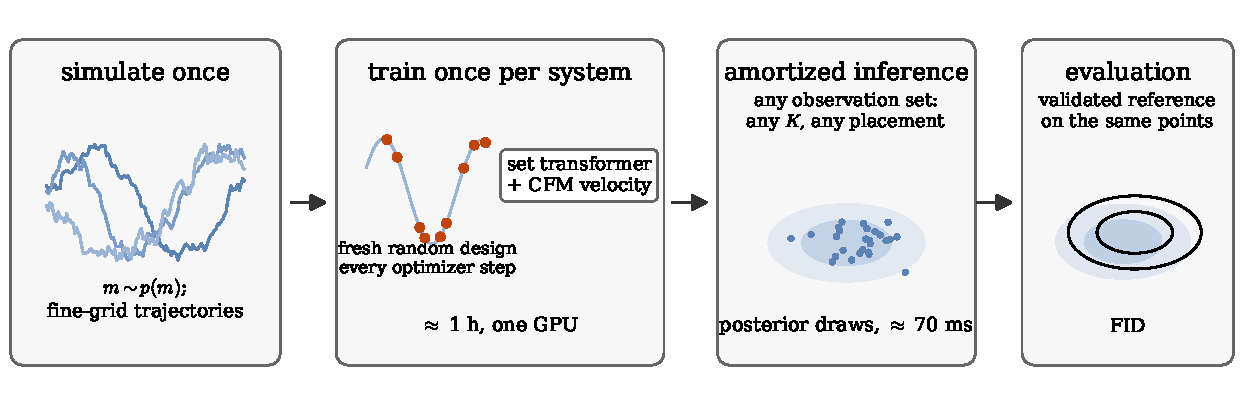
\includegraphics[width=\linewidth]{figs/overview.pdf}
\caption{\textbf{Overview.} Parameters drawn from the prior are simulated once on a fine grid (left).
Training fits a conditional flow-matching posterior with a set-transformer encoder and draws a fresh
random observation design at every optimizer step (Secs.~\ref{sec:arch}, \ref{sec:recipe}). The
trained network returns posterior samples for any observation set of the experiment, at any number
and placement of points. Accuracy is measured against exact or validated reference posteriors computed
on the same observed points (Sec.~\ref{sec:protocol}).}
\label{fig:overview}
\end{figure}

Figure~\ref{fig:overview} gives an overview of our approach. This section defines each element in
turn.

\subsection{Problem formulation}

Consider a dynamical system that depends on a parameter vector $m \in \R^{d}$ with a known prior
$p(m)$, uniform on a box in all our benchmarks. The system produces a state trajectory $x(t)$ through
an ODE $\dot{x} = f(x; m)$, an SDE $dx = f(x;m)\,dt + \sigma(x;m)\,dW_t$, or a spatially discretized
PDE. The trajectory is observed through a noisy channel at $K$ points:
\begin{equation}
  y_i = h\bigl(x(t_i)\bigr) + \varepsilon_i, \qquad
  \D = \{(t_i, y_i)\}_{i=1}^{K}.
  \label{eq:obs}
\end{equation}
We call $\D$ the \emph{observation set} of one experiment; it is the entire input to inference.
Training and evaluation involve many independently simulated observation sets, each paired with the
parameter that generated it. The observation operator $h$ may expose only part of the state. In our
benchmarks it exposes only the price of an asset while the stochastic volatility is latent, only the
membrane voltage of a neuron while the gating variables are latent, or only three spatial sensors of
a PDE field. The target is the posterior $p(m \mid \D) \propto p(\D \mid m)\, p(m)$.

Three assumptions delimit the setting. The parameter is finite- and low-dimensional ($d = 2$--$5$ in
every benchmark), with a prior that factorizes across components and has tractable marginal CDFs
(uniform boxes throughout; the construction extends to any such prior). The simulator can be run
forward cheaply and repeatedly, and nothing else is required of it: no likelihood evaluations and no
gradients. The observation times and sensor indices are known exactly, and the measurement noise
$\varepsilon_i$ is independent across observations with a known per-system law.

Although the posterior itself is intractable, sampling from the \emph{joint} distribution of
parameters and data is easy: draw $m_j \sim p(m)$, simulate the system, apply the observation channel.
This yields arbitrarily many training pairs $(m_j, \D_j)$, and a conditional generative model trained
on these pairs approximates the posterior for every observation set simultaneously. The cost of
inference moves into a one-time training phase, and inference for a new observation set is a single
forward pass. We impose one requirement beyond standard amortization: a single trained network must
remain correct for any number $K$ and any placement of observation times (and, for PDEs, sensor
positions). Formally, for every subset $S$ of the measurement points of one experiment the network
must approximate $p(m \mid S)$, and the family of answers must be coherent; in particular, the
posterior must widen when points are removed. We call this requirement \emph{design amortization}. It
produces the object that sequential refinement and Bayesian experimental design consume, since both
rank candidate observation schedules by the posteriors the schedules would produce.

\subsection{Posterior sampling by conditional flow matching}
\label{sec:method}

We represent the posterior as a \emph{transport} rather than as a density formula: a learned,
data-conditioned deformation that carries a fixed reference distribution onto the posterior. Sampling
draws from the reference and applies the deformation. There is no normalizing constant to compute and
no invertibility constraint on the network. The deformation is defined implicitly as the flow of a
velocity field, and the field is fitted by ordinary least-squares regression on simulated pairs. This
construction is conditional flow matching \citep{lipman2023}.

\paragraph{Normalization.} We first reparametrize the parameters component by component,
\begin{equation}
  m \;\longmapsto\; \Phi^{-1}\!\bigl(F_{\text{prior}}(m)\bigr) \in \R^{d},
  \label{eq:probit}
\end{equation}
where $F_{\text{prior}}$ collects the marginal prior CDFs and $\Phi$ is the standard normal CDF. In
the new coordinates the prior is exactly $\N(0, I)$ and the box constraints disappear. The
uninformative limit then costs nothing: when the data carry no information, the posterior is the
reference and the transport is the identity. From here on we work in these coordinates and keep the
symbol $m$ for the parameter in them. The inverse of \eqref{eq:probit} is applied exactly once, at the
end of sampling, to return the draws on the original scale.

\paragraph{Training objective.} A \emph{virtual time} $\tau \in [0, 1]$ indexes the transport. This is
an algorithmic variable with no relation to the physical time $t$ at which the system is observed:
$t$ appears only inside observation sets, and $\tau$ only in the transport. Subscripts in $\tau$
denote the position along the transport path. The endpoint $m_1$ is a parameter drawn together with
its observation set $\D$. The start $m_0 \sim \N(0, I)$ is pure reference noise, not the transform of
any parameter; it is the raw material that the transport turns into a posterior draw at $\tau = 1$.
Between them lies the training interpolation $m_\tau = (1 - \tau)\, m_0 + \tau\, m_1$. The velocity
network learns the direction of this path by regression:
\begin{equation}
  \mathcal{L}(\theta) =
  \E_{\,m,\D,\; m_0 \sim \N(0,I),\; \tau \sim U[0,1]}
  \bigl\| v_\theta(m_\tau,\, \tau,\, \D) - (m_1 - m_0) \bigr\|^2 .
  \label{eq:cfm}
\end{equation}
The minimizer of \eqref{eq:cfm} is the marginal velocity field, whose flow transports $\N(0, I)$ at
$\tau = 0$ to $p(m_1 \mid \D)$ at $\tau = 1$ \citep{lipman2023}. Sampling draws $m_0 \sim \N(0, I)$,
integrates $dm/d\tau = v_\theta(m, \tau, \D)$ from $\tau = 0$ to $1$, and maps the endpoint back
through the inverse of \eqref{eq:probit}. The numerical settings of this integration are not a detail:
Sec.~\ref{sec:recipe} states them and reports a case where the usual grid fails. The same estimator
family, with a different conditioning architecture, is available in \texttt{sbi} as flow-matching
posterior estimation (FMPE) \citep{wildberger2023}. Our package differs in the input representation,
not in the generative engine.

No stage requires likelihood evaluations, simulator gradients or per-instance optimization. The
simulator runs forward only, during the generation of the training set.

The training objective is consistent in the following sense.

\begin{proposition}[consistency]
Let $(m, \D) \sim p(m)\,p(\D \mid m)$ and let $m_1$ be given by \eqref{eq:probit}. Minimize the loss
\eqref{eq:cfm} over all measurable velocity fields. Then for $p(\D)$-almost every $\D$ the flow of the
minimizer transports $\N(0, I)$ at $\tau = 0$ to the conditional law $p(m_1 \mid \D)$ at $\tau = 1$.
Equivalently, the sampling procedure above draws exactly from the posterior
\citep{lipman2023, wildberger2023}.
\end{proposition}

The proposition is an idealization. A finite network, a finite simulation budget and a numerical
solver remove every calibration guarantee, and the residual error becomes an empirical quantity.
Sec.~\ref{sec:protocol} builds the instruments that measure it.

\section{Conditioning architecture}
\label{sec:arch}

The velocity field $v_\theta(m, \tau, \D)$ is conditioned on an observation set of time-stamped
measurements. Three properties of that set drive the architecture. The number of observations $K$
varies from experiment to experiment, by two orders of magnitude in the variable-design setting. The
observation times are arbitrary real numbers, in general not equally spaced, so positional schemes for
uniform sequences do not apply. The times carry all ordering information, so the output must not
depend on the storage order of the observations. These properties rule out the fixed-length-vector
conditioners of NPE implementations. A transformer that operates on one feature vector per observation
meets all three. We call that feature vector a \emph{token}.

\begin{figure}[t]
\centering
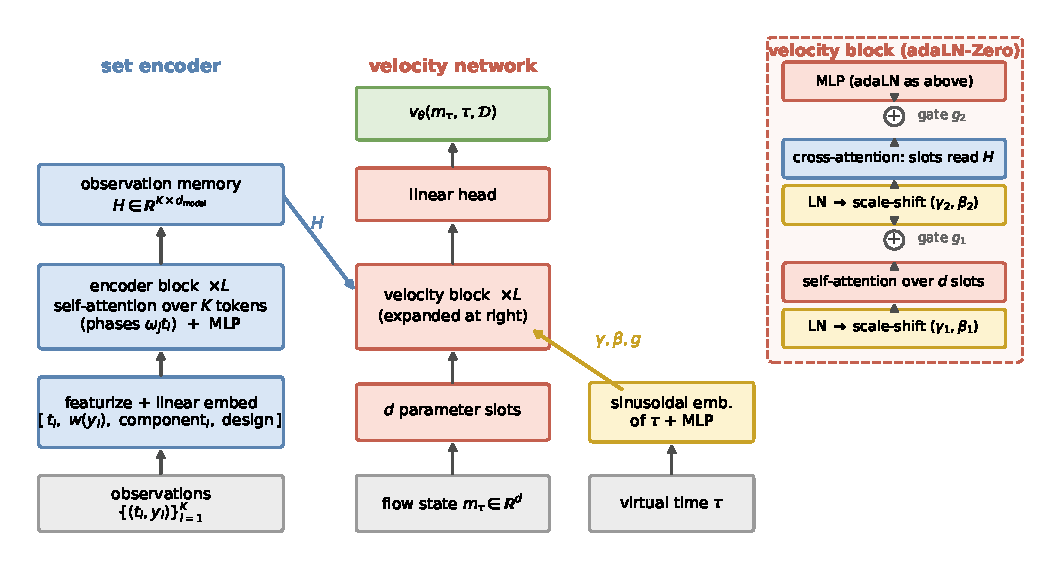
\includegraphics[width=0.95\linewidth]{figs/arch.pdf}
\caption{\textbf{Architecture.} Arrows show the data flow, bottom to top. Left: each observation is
featurized and linearly embedded into one token. $L$ transformer encoder blocks produce a memory $H$ of
$K$ encoded states, whose attention phases come from the physical observation times
(Sec.~\ref{sec:trope}). Middle: the $d$ components of the flow state $m_\tau$ form $d$ parameter-slot
tokens; $L$ velocity blocks and a linear head map them to the velocity $v_\theta$. Right: one velocity
block. It has self-attention across the parameter slots, cross-attention that reads the observation
memory $H$, and an MLP. Layer normalization with scale-shift $(\gamma, \beta)$ precedes each part, and
a gated residual connection ($g$, marked $+$) follows it. A zero-initialized map produces the triples
$(\gamma, \beta, g)$ from the virtual time $\tau$, so the untrained block is the identity
\citep{peebles2023}.}
\label{fig:arch}
\end{figure}

\subsection{Overall scheme}
\label{sec:scheme}

The network evaluates $v_\theta(m, \tau, \D)$, where $m$ is the normalized parameter vector partway
along its transport path (the interpolation $m_\tau$ at training time, the current ODE state at
sampling time) and $\tau$ is the virtual time of the transport. We follow the encoder--decoder pattern
of conditional flow-matching and diffusion models: the data are encoded once, and a decoder combines
that encoding with the object being generated,
\begin{equation}
  v_\theta(m, \tau, \D) \;=\; \mathrm{Dec}\bigl(m,\; \tau,\; \mathrm{Enc}(\D)\bigr).
  \label{eq:encdec}
\end{equation}
The types are explicit. $\mathrm{Enc}$ maps the observation set, the $K$ time-stamped measurements of
one experiment, to a memory of $K$ vectors, $\mathrm{Enc}(\D) \in \R^{K \times d_{\mathrm{model}}}$,
computed once per observation set. $\mathrm{Dec} : \R^{d} \times [0,1] \times \R^{K \times
d_{\mathrm{model}}} \to \R^{d}$ combines the current transport point and the virtual time with that
memory. Two differences from the image and text instances of this pattern determine the concrete form
(Fig.~\ref{fig:arch}). First, the conditioning is not a fixed-size embedding but an observation set of
variable size $K$. $\mathrm{Enc}$ is therefore a transformer over per-observation tokens, and its
output is a \emph{memory} of $K$ encoded states rather than one pooled vector. $\mathrm{Dec}$ reads
the memory by cross-attention, the one standard mechanism that does not depend on $K$. Second, the
generated object is a short vector of $d$ parameters, not an image, so the decoder is small. The $d$
components of $m$ are $d$ tokens, and self-attention among them expresses posterior correlations, such
as the ridge of the Fisher--KPP posterior or the drift--volatility coupling of GBM. The virtual time
$\tau$ enters every block through zero-initialized adaptive layer normalization (adaLN-Zero), the
conditioning mechanism of diffusion transformers \citep{peebles2023}, so that the untrained network is
an identity-like map.

On the encoder side, each observation $i$ is described by a few features, and a learned linear map
lifts them to the model width. There are four features: the time $t_i$; the transformed value
$w(v_i)$, where $v_i$ is the observed value in the coordinate the problem declares and $w$ is the
learnable monotone map of Sec.~\ref{sec:features}; an index of the sensor or state component that
produced the value (a multivariate state gives one token per observed component per time); and the
design-size feature of Sec.~\ref{sec:features}. Sec.~\ref{sec:trope} describes the attention mechanism
through which the tokens interact, and Sec.~\ref{sec:features} describes the choice of features.

This scheme is the survivor of a sequence of measured alternatives, and the failed alternatives remain
in the package as reproducible controls. All sizes are configuration parameters. One configuration
(width 64, four heads, three blocks per side) serves every experiment in this report. At the
training-set sizes we use, models of this scale are sufficient: doubling width and depth changes no
benchmark result. Nothing in the construction caps the scale.

\subsection{Attention phases from observation times}
\label{sec:trope}

We adapt rotary position embeddings, the standard positional scheme of modern transformers
\citep{su2024}, to irregular time sampling.

\paragraph{Rotary embeddings.} We recall the classical construction. Token states
$x_1, \dots, x_K \in \R^{d_{\mathrm{model}}}$ enter an attention layer. Each head computes
\begin{equation}
  q_i = W_Q x_i, \qquad k_i = W_K x_i, \qquad u_i = W_V x_i,
  \qquad W_Q, W_K, W_V \in \R^{d_h \times d_{\mathrm{model}}},
\end{equation}
and token $i$ aggregates the other tokens with weights
$a_{il} = \operatorname{softmax}_l\bigl(\hat q_i^\top \hat k_l / \sqrt{d_h}\bigr)$. The hats mark
position-modulated vectors: each query and key is split into $d_h/2$ planar blocks
$q_i^{(j)} \in \R^2$, and block $j$ is rotated by an angle set by a per-token scalar $\phi_i$,
\begin{equation}
  \hat q_i^{(j)} = R(\omega_j \phi_i)\, q_i^{(j)}, \qquad
  \hat k_i^{(j)} = R(\omega_j \phi_i)\, k_i^{(j)}, \qquad
  R(\phi) = \begin{pmatrix} \cos\phi & -\sin\phi \\ \sin\phi & \cos\phi \end{pmatrix}.
  \label{eq:trope}
\end{equation}
In the classical scheme the scalar is the integer position of the token in the sequence,
$\phi_i = n_i$, and the frequencies form a geometric progression across blocks,
$\omega_j = \omega_{\max} (\omega_{\min}/\omega_{\max})^{(j-1)/(d_h/2-1)}$: high-frequency blocks
resolve neighboring positions and low-frequency blocks resolve long ranges. Rotations preserve inner
products up to the relative angle,
\begin{equation}
  \hat q_i^{\top} \hat k_l
  \;=\; \sum_{j=1}^{d_h/2} \bigl(q_i^{(j)}\bigr)^{\top} R\bigl(\omega_j (\phi_l - \phi_i)\bigr)\, k_l^{(j)},
  \label{eq:ropeinv}
\end{equation}
so every attention logit depends on the positions only through the differences $\phi_l - \phi_i$.
This gives relative position awareness with no positional parameters.

\paragraph{Physical time as the phase.} For irregularly sampled data the integer position has no
meaning. Our generalization is direct: we set $\phi_i = t_i$, the physical time stamp of observation
$i$, and choose the frequency range so that the periods $2\pi/\omega_j$ span from the finest
observable time gap to several times the horizon. Nothing else changes. By \eqref{eq:ropeinv}, every
logit now depends on the time stamps only through the differences $t_l - t_i$. Time-aware attention
models for irregular clinical and event series make the same substitution in other positional schemes
\citep{horn2020, shukla2021}. Two consequences follow. The encoder is exactly permutation-invariant:
relabeling the tokens leaves the right-hand side of \eqref{eq:ropeinv} unchanged, which we verified
numerically to $10^{-8}$. And variable designs need no positional bookkeeping. The phases enter only
the self-attention of the encoder. The cross-attention from the parameter slots to the observation
memory is unmodified attention, because the parameter slots carry no time stamp and the memory states
already encode the temporal structure.

Integer positions create an implicit train/test contract on token placement. In a control experiment
we trained a model on spread-out subsampled positions and evaluated it on contiguously packed ones.
The posterior acquired substantial biases while every component stayed individually correct. With
physical-time phases this contract does not exist.

\subsection{Input features}
\label{sec:features}

The remaining design choices concern the content of the tokens. Four of them matter: the coordinate of
the observed value, and three learnable modules, namely a transform of the observed values, an
optional increment-based token construction for directly observed diffusions, and an explicit
design-size feature. Each module is a few lines of code. Each repairs a measured failure in the
conditioning of the numbers that the set encoder receives, and each repair is a learnable module
rather than a problem-specific transformation.

\paragraph{Value coordinate.} The problem declares the coordinate in which the observed value enters
the token: the value itself, or its logarithm. The package has no default for this choice. The rule is
simple: use the coordinate in which the observation noise is additive. For log-normal assay noise this
is the logarithm. The learnable transform of the next paragraph does not replace this rule. With raw
values under log-normal noise, populations below about $0.05$ are compressed into an interval below
the resolution of the network, although the noise model measures their logarithm to $\pm 0.1$. On such
observation sets the posterior centre misses by several posterior widths. We measured this on the
Lotka--Volterra system of the \texttt{sbibm} benchmark: changing the token value from the raw
population to its logarithm improves the median classifier two-sample test against MCMC from $0.79$
to $0.73$. All measurements in this report use raw values.

\paragraph{Value transform.} The state variables of the benchmark systems live on very different
scales. Some of them (prices, concentrations, populations) are multiplicative: the information sits in
relative changes, and the natural coordinate is logarithmic. Ignoring this is costly. On GBM, raw
price tokens under global standardization force the network to divide squared increments by squared
levels internally, and the result is a persistent volatility bias that training does not remove. We
do not prescribe coordinates per problem. Instead, each value enters its token through a learned
monotone map,
\begin{equation}
  w(x) \;=\; \sum_{k=1}^{S} a_k \,\operatorname{sign}(x) \log\!\bigl(1 + |x| / s_k\bigr),
  \qquad a_k \ge 0.
  \label{eq:warp}
\end{equation}
Each basis function is linear for $|x| \ll s_k$ and logarithmic for $|x| \gg s_k$, so the family
contains the identity, the signed logarithm and every compression in between. The weights are
positive, so $w$ is monotone by construction. Every candidate compression is present from
initialization: training only reweights fixed nonlinearities, and the downstream network can use the
helpful coordinate from the first optimizer step. The scales $s_k$ sit on a fixed geometric grid of
$S = 8$ octaves that covers the dynamic range of the data. One setting serves all fourteen systems,
with no per-problem adjustment.

\paragraph{Comparison with other learnable transforms.} We compare this structure with simpler
learnable alternatives on geometric Brownian motion, where the correct coordinate (the log-price) is
known, so that a failure to find it is visible against the closed-form posterior. A generic two-layer
MLP on the raw values and a random-Fourier-feature map both fail to find the coordinate at a matched
budget. A free-form map must discover the shape and the scale of the compression at the same time,
with gradients that arrive through the whole downstream network; in practice it does not. The
Yeo--Johnson power transforms \citep{yeo2000} also fail. This is a classical one-parameter family, in
essence $x \mapsto ((1+|x|)^{\lambda} - 1)/\lambda$ with sign symmetry, which passes through the
identity at $\lambda = 1$ and tends to the logarithm as $\lambda \to 0$. Trained end-to-end, $\lambda$
never leaves its initialization: a single global exponent must cross a gradient plateau before the
downstream network learns anything that rewards the move. The parametrization decides the outcome,
not the hypothesis class. The mixture \eqref{eq:warp} finds the coordinate reliably, and the trained
weights concentrate on the small-scale components: the model learns the log-price.

\paragraph{Increment features for directly observed diffusions.} For scalar SDEs whose state is
observed directly, with no latent components, the package offers a second token construction. After a
sort by time, consecutive observations contribute
\[
  \bigl[\,t_{(i)},\; w(y_{(i)}),\; \Delta w_i,\; (\Delta w_i)^2,\; w_t(\Delta t_{(i)})\,\bigr],
  \qquad \Delta w_i = w(y_{(i+1)}) - w(y_{(i)}).
\]
The motivation is elementary. For a Markov observed process the likelihood factorizes over
consecutive pairs, transition densities of diffusions depend on increments and gaps, and squared
increments carry the quadratic-variation information that identifies diffusion coefficients. This is
an inductive bias of the same kind as convolutions for images: useful where its assumption holds, not
a requirement of the method. The point-token path of Sec.~\ref{sec:scheme} is fully general.

The rule for choosing between the two constructions is: use increment tokens exactly when the observed
process is Markov. We tested the rule in both directions. An increment-token model transfers across
Markov systems without adjustment. On the Heston model the observed price is not Markov, because the
volatility is latent, and there increment and point tokens perform identically, as the factorization
argument predicts. A per-problem flag selects the construction.

Two normalization details matter for processes with jumps, where squared increments within one
observation set span several orders of magnitude. A running feature normalization then takes its scale
from the rare outliers and never converges: the representation drifts during training, the flow trains
against a moving target, and the Merton jump-diffusion acquires a substantial volatility bias. Probes
of the encoder show a failure of representation stability, not of extraction; the failing
configuration encodes robust volatility statistics as well as the healthy one does. Two repairs
follow. First, the increment features are logarithmically compressed before normalization. This is a
near-identity on systems without jumps, since $\log(1+x) \approx x$ for small $x$, and in our
experiments it removes the bias. Second, a smaller residual remains, whose mechanism is a
jump-classification threshold that floats with the unknown volatility. To remove it, we let the
normalization adapt to the observation set. Robust summary statistics $s$ of the set are pooled over
the non-padding positions, and a zero-initialized MLP maps them to per-channel scale and shift
corrections,
\begin{equation}
  h_c \;\mapsto\; \bigl(1 + \gamma_c(s)\bigr)\, h_c + \beta_c(s).
  \label{eq:film}
\end{equation}
This is a feature-wise affine modulation, FiLM in the terminology of \citet{perez2018}. It removes the
residual as well as a hand-crafted per-observation-set rescaling does. Three conditions are necessary
for it to help: zero initialization, modulation applied \emph{after} the running normalization, and
pooled statistics that exclude the padding positions.

\paragraph{Design size.} The number of observations governs the posterior width: in regular models the
error scales as $K^{-1/2}$. Softmax attention computes normalized weighted means and is therefore
almost invariant to the size of the set it aggregates. Probes of the encoder confirm the mechanism.
Every variant we tested recovers posterior-mean statistics from the pooled output, but how well the
pooled output encodes $\log K$ varies widely across variants, and it ranks them exactly in the order
of their width errors. We therefore supply this one number as an explicit feature, $\log K$ in every
token. This removes most of the width error at dense designs; the design-resampling training procedure
of Sec.~\ref{sec:recipe} removes the rest. A few learned register tokens \citep{darcet2024} give the
same effect without an explicit feature.

\section{Training procedures}
\label{sec:recipe}

\paragraph{Sampler.} All measurements in this report sample with the midpoint scheme, 20 steps, on a
uniform time grid. We fixed the step count by a convergence check on the benchmark suite: fourth-order
Runge--Kutta with three times as many steps changes no benchmark statistic. This check holds for the
posteriors of the suite, which are $4$--$107$ times narrower than the prior at the median instances.
It does \emph{not} hold for much narrower posteriors. We found this later, on the Lotka--Volterra
system of \texttt{sbibm} with 20 observations, where the posterior is $20$--$280$ times narrower than
the prior. Near $\tau = 1$ the Jacobian of the field is about $-1/(1-\tau)$ until $1 - \tau$ is of the
order of the posterior width in the normalized coordinates, so a uniform grid of $n$ steps cannot
resolve a posterior narrower than about $1/n$ with any explicit scheme. The samples then have the
correct marginal widths and the wrong joint structure. For the exact flow-matching field of a Gaussian
target of width $0.01$, the uniform grid with 20 midpoint steps gives a classifier two-sample test of
$0.92$ against the target ($0.5$ means indistinguishable), and fourth-order Runge--Kutta with 50
uniform steps gives $0.60$. A grid whose steps shrink towards $\tau = 1$ as $(1 - i/n)^3$ gives $0.50$
with the same 20 midpoint steps, down to a width of $0.003$. On the trained Lotka--Volterra flow the
same change moves the test from $0.80$ to $0.57$ at no extra cost. The package now provides both
grids, and the caller names the grid, the scheme and the step count in every sampling call. The
shrinking grid is the choice for posteriors that can be much narrower than the prior.

\paragraph{Optimizer.} Evaluation uses an exponential moving average of the training weights (decay
$0.999$). The optimizer is Muon \citep{jordan2024}: a Newton--Schulz iteration orthogonalizes the
momentum of every two-dimensional weight before the update, and Adam updates the biases,
normalizations and embeddings. The step size follows a measured batch-size rule $\eta(B)$
(Appendix~\ref{app:optmeas}). The schedule is cosine with linear warmup, and the gradients are clipped.
At every optimizer step the virtual times are drawn afresh, stratified over $[0,1]$:
$\tau_i = (i - 1 + u_i)/B$ for a batch of size $B$, with $u_i \sim U[0,1]$ i.i.d., $i = 1, \dots, B$.
Fresh reference noise $m_0$ is drawn with them, so no pairing of observation sets and virtual times
repeats. For fixed-design problems the training set has $n$ simulated observation sets, and training
runs for a fixed number of epochs over it; the calibration-screen gallery of
Appendix~\ref{app:systems} uses $n = 40{,}000$ simulations and 35 epochs.

\paragraph{Design amortization.} Training data are simulated once on a fine grid. Observation designs
are then resampled \emph{from the stored fine trajectories at every optimizer step}. The procedure has
three parts, each fixed by a controlled comparison on GBM, Ornstein--Uhlenbeck and FitzHugh--Nagumo:
\begin{enumerate}
  \item \emph{Fresh designs at every step.} Each step re-draws the observation subset of each
  trajectory. Design memorization becomes impossible, and one simulation serves arbitrarily many
  designs. The alternative, one fixed design per trajectory, closes the dense-design error at long
  budgets but overfits the design set; in our experiments it gives overconfident posteriors at sparse
  $K$.
  \item \emph{The design-size law.} $K$ is drawn $50\%$ log-uniform on $[K_{\min}, K_{\max}]$ and
  $50\%$ uniform on the dense half of the range. Log-uniform sampling alone puts too little mass at
  large $K$ and leaves dense designs under-trained. The mixture removes the effect.
  \item \emph{Budget scaling.} For higher accuracy, we scale simulations and optimizer steps together
  at a constant number of epochs. In our experiments the residuals then decrease steadily with this
  single budget variable, whereas passes over reused observation vectors eventually destroy accuracy.
  This is why the scaling must be joint.
\end{enumerate}
With this procedure, the posterior width matches the exact per-design posterior closely and uniformly
over the whole range of design sizes.

\paragraph{Budgets and stopping.} Step budgets have deliberate slack, and validation chooses the
shipped weights. Training monitors a validation set, built by the same tools as the test evaluation
sets from disjoint seeds. The final weights are replaced by the best monitored checkpoint only when
two conditions hold: the improvement must exceed the resolution of the monitor, and the monitored
value must sit at least three floors above that resolution. A monitor that ranks values of its own
resolution returns noise in both directions. With that margin, overshooting a budget costs time and
never quality, so the step budget is not a per-system quantity to tune. Appendix~\ref{app:optmeas}
gives the measurements behind the margin, including the two failure modes of the naive
best-checkpoint rule.

\begin{figure}[t]
\begin{lstlisting}[style=he]
# ---- training a design-amortized posterior ---------------------------------
m_all, X_all = simulate(prior, n)      # full fine-grid trajectories, once
theta_best, F_best = None, inf
for step in range(T):                  # step budget T, set with slack
    m1, X = batch(m_all, X_all, B)     # stored trajectories, reused
    tokens = tokenize(X, fresh_designs(B))  # per trajectory: K from the mix
                                            #   law, K random (time, sensor) points
    tau = stratified(B)                # fresh virtual times, stratified on [0,1]
    m0 = randn(B, d)                   # fresh reference noise
    z = (1 - tau) * m0 + tau * m1
    loss = norm(v(z, tau, Enc(tokens)) - (m1 - m0)) ** 2
    muon_step(loss, lr=eta(B))         # batch step rule, cosine schedule
    ema.update()
    if step % Delta == 0:              # score the EMA weights on validation
        F = monitor(ema, val)
        if F < F_best: theta_best, F_best = copy(ema), F
# ship the best checkpoint only when it clears the monitor's own resolution
if F - F_best > phi and F_best >= kappa * phi: return theta_best
return ema
\end{lstlisting}
\vspace{1.5mm}
\begin{lstlisting}[style=he]
# ---- inference: n posterior draws for one observation set S ----------------
C = Enc(tokenize(S))                   # encode once; any size, any placement
z = randn(n, d)                        # or the learned base, where enabled
for tau, h in grid(L, kind):           # L steps; kind = "uniform" or "late"
    z_mid = z + h/2 * v(z, tau, C)     # midpoint scheme, 2 evaluations per step
    z = z + h * v(z_mid, tau + h/2, C)
return denormalize(z)
\end{lstlisting}
\caption{\textbf{Pseudocode} of training (top) and inference (bottom). The step rule $\eta(B)$ is that
of Sec.~\ref{sec:recipe}, the monitor period is $\Delta = T/24$, and the resolution multiple is
$\kappa = 3$ with monitor floor $\varphi$ (Appendix~\ref{app:optmeas}). The measurements of this
report use $L = 20$ steps on the uniform grid. The caller names $L$, the scheme and the grid in every
sampling call (Sec.~\ref{sec:recipe}).}
\label{fig:pseudocode}
\end{figure}

\begin{figure}[t]
\begin{lstlisting}[style=he]
import torch
from amortix import FlowPosterior, DESIGN_ZOO

prob = DESIGN_ZOO["heston"]()             # or any DesignProblem subclass; the class
                                          #   declares value_coord ("raw" or "log")
post = FlowPosterior(prob)                # embedding/RoPE resolve from the class
post.fit(n_train=120_000, steps=72_000,   # about 1 h on one GPU
         retokenize=prob.make_retokenizer())  # fresh designs at every step

gen = torch.Generator().manual_seed(0)
m, raw = prob.simulate(1, gen)            # here: one synthetic observation set
tidx, cidx = prob.sample_design(gen, 20)  # 20 (time, sensor) points
tokens = prob.tokens_for(raw[0], tidx, cidx, gen)
draws = post.sample(tokens, n=2000, n_steps=20, solver="midpoint",
                    t_grid="late")       # [2000, d] draws, milliseconds
\end{lstlisting}
\caption{\textbf{Usage.} The interface for the procedure of Fig.~\ref{fig:pseudocode}: a benchmark
system from the design zoo, training, and posterior draws for one observation set. The sampling
settings have no default values. Appendix~\ref{app:package} maps the terms of this report to the
package options.}
\label{fig:usage}
\end{figure}

\section{Evaluation methodology}
\label{sec:protocol}

We measure accuracy against reference posteriors computed on the same observed points. Every number in
this report therefore says how far the posterior of the network is from the posterior that the data
imply. It never says how well the network satisfies a self-consistency condition.

\subsection{Reference posteriors as the record}
\label{sec:refs}

\paragraph{Metric.} Where a tractable likelihood exists, we compare distributions on the same observed
points. The headline statistic is one number per observation set: the squared Fr\'echet distance
between Gaussian fits of the two sample sets, in reference-normalized coordinates where each parameter
is divided by the standard deviation of the reference posterior,
\begin{equation}
  d_F^2 \;=\; \lVert \mu_a - \mu_r \rVert^2
  + \operatorname{tr}\!\bigl(\Sigma_a + \Sigma_r
  - 2\,(\Sigma_r^{1/2} \Sigma_a \Sigma_r^{1/2})^{1/2}\bigr).
  \label{eq:fid}
\end{equation}
This is the construction of the FID score in the image-generation literature, and we use that name.
The quantity is dimensionless only after a choice of scale, and we use two scales. Let $\sigma_{r,i}$
be the standard deviation of the reference posterior in coordinate $i$ and $\Delta_i$ the width of the
prior box. Then
\begin{equation}
  \FIDsd = d_F^2\bigl(\{m_a/\sigma_r\},\ \{m_r/\sigma_r\}\bigr), \qquad
  \FIDpr = d_F^2\bigl(\{m_a/\Delta\},\ \{m_r/\Delta\}\bigr).
  \label{eq:fidnorm}
\end{equation}
In $\FIDsd$ every coordinate is divided by the standard deviation of the reference posterior. This is
the default, and an unadorned FID in this report means $\FIDsd$. In $\FIDpr$ every coordinate is
divided by the prior range. The two answer different questions: error relative to what the data
determine, and error relative to the scale of the problem. A model of fixed absolute accuracy reads
very differently in the two scales where the posterior is narrow (Sec.~\ref{sec:design-amortization}).

FID is zero for a perfect match and dimensionless, and it combines the three ways a posterior can be
wrong: location, width and orientation. For scale: a bias of $0.1$ reference-sd in each of $d$
dimensions gives FID $0.01\,d$, and a posterior $30\%$ too wide in one dimension gives FID
$\approx 0.09$. Where the direction of a failure matters, we also quote the per-parameter
decomposition, because a posterior that is too wide is conservative while a posterior that is too
narrow misleads without a warning. The decomposition gives the signed posterior-mean error in
reference-sd units (\emph{bias}) and the ratio of standard deviations (\emph{width}); a width of $1$
is exact, above one is conservative, below one is overconfident.

\paragraph{Admission of a reference.} The engines of the next paragraph build the references, and
Appendix~\ref{app:refs} gives the construction. A second chain from a well-separated start validates
every MCMC reference, and a reference is used only when its two chains agree. The between-chain
discrepancy of the posterior mean, in posterior-sd units, is the floor below which nothing can be
measured, and we quote that floor next to the value of the model throughout. The floor scales with the
chain length. The Merton jump-diffusion needs $2 \times 10^5$-draw chains to clear it: two chains then
agree to $0.016$~sd in the median and $0.060$ at worst. A system whose chains do not converge at any
affordable length is reported under the calibration screen instead. After the engine upgrades of the
next paragraph, no system of the suite is in that state.

\paragraph{Reference samplers.} For nonlinear ODEs and SDEs, trustworthy reference posteriors are a
task in themselves. For every system we tested several approaches and adopted the per-problem methods
below; the structure of the likelihood decides the sampler. Where a closed form exists, we draw the
posterior exactly (linear-Gaussian; GBM through its conjugate structure). Where the likelihood is
exact but the posterior is not, adaptive Metropolis suffices for the well-conditioned systems:
Ornstein--Uhlenbeck, Cox--Ingersoll--Ross (through its noncentral $\chi^2$ transitions), SEIR,
Merton, pharmacokinetics and Fisher--KPP. FitzHugh--Nagumo and Hodgkin--Huxley have needle-thin or
multimodal posteriors. Their sharpest evaluation instances concentrate the posterior to $0.4\%$ and
$1.0\%$ of the prior range in the narrowest coordinate, and adaptive Metropolis chains from separated
starts disagreed on them by hundreds of posterior standard deviations. These two systems therefore
use nested sampling with \texttt{dynesty} \citep{skilling2006,speagle2020}. On the median instances
their posteriors are unremarkable ($3$--$30\times$ narrower than the prior); the needle is a property
of the sharp tail, and there chain methods fail. Double well and polynomial drift have no transition
density in closed form, so their likelihood is an unbiased bridge estimate \citep{durham2002} inside
pseudo-marginal MH \citep{andrieu2010}. Stochastic Lotka--Volterra and Heston are the two systems
whose likelihood is available only as a Monte-Carlo estimate, not as a computable number. Nested
sampling assumes a deterministic likelihood and does not apply to them. Their references come from
adaptive tempered SMC \citep{delmoral2006} over an unbiased particle estimate, admitted by population
doubling. The estimate enters a pseudo-marginal kernel, so its variance is a property of the
reference: the log of an unbiased estimator is biased downward by about half its variance, and where
that variance varies over the parameter space the bias tilts the posterior. Both systems therefore
run at a particle count at which the spread of the estimator is a fraction of a nat, which we verify
by repeated estimates at fixed parameters.

\paragraph{Three checks.} Every reference passes three checks before use. Two independent runs must
agree below $0.25$ posterior sd. The likelihood must reproduce the simulator: on noiseless data its
value at the generating parameters is zero to machine precision. The generating parameters must lie
inside the posterior. The three checks are not redundant; each one caught a wrong likelihood in this
work that the other two passed. The third check catches a reference that describes a different model
than the simulator. Across the frozen evaluation sets of the suite, the generating parameters sit at
a median $0.5$--$0.8$ posterior sd from the reference mean, and only $0$--$1\%$ of the coordinates lie
beyond three (Appendix~\ref{app:optmeas}).

Heston is the sharpest case of the third check, because the first two checks do not see the failure.
We first built its reference from the idealized transition of the continuous-time model. That is a
different process from the one that generated the data: the simulator integrates the variance by
clamped Euler, and past the Feller condition the variance spends real time pinned at zero. The
discrepancy grows with the vol-of-vol $\xi$. On instances generated with $\xi \approx 0.9$ the
reference placed $\xi$ near $0.27$ at half the true width, and the two independent chains agreed on
that wrong answer to $0.17$~sd. Only the generating parameter, $8.1$ posterior sd outside its own
reference, exposed the defect. We replaced the idealized transition by a bootstrap particle filter
that runs the update rule of the simulator itself, admitted by two closed forms in the $\xi = 0$
limit. The worst deviation moved to $2.6$~sd, the two-chain agreement tightened to $0.06$~sd, and the
floor of the set halved. Against the corrected reference, the dependence of Heston on model size is
unremarkable (Sec.~\ref{sec:results}).

\paragraph{Resolution of the estimator.} Both sample sets are finite, so \eqref{eq:fid} is positive
even for a perfect posterior, and the size of that offset sets what the metric can resolve. We
measured it directly by drawing \emph{two independent sample sets from the same exact GBM posterior}
and scoring one against the other. The median FID is $0.0157$ at $500$ samples, $0.0038$ at
$2{,}000$, $0.0009$ at $8{,}000$ and $0.0002$ at $32{,}000$. This is a clean $1/n$, as the estimation
error of the fitted means and covariances predicts. Two consequences follow. Differences below
$\approx 0.005$ at $n = 2{,}000$ ($\approx 0.002$ at the $4{,}000$ draws that score the evaluation
sets of Table~\ref{tab:main}) are not resolved; we report values in that range as ``at the resolution
limit'' and do not compare them. The best values in this report sit above the limit, not at it. The
design-amortized GBM model reads $0.0107$ at $n = 2{,}000$, $0.0100$ at $8{,}000$ and $0.0072$ at
$32{,}000$ on the same evaluation set. After subtraction of the estimator offset, its excess over the
reference is $\approx 0.007$ at every sample size. This is a real error of the model, not an artifact
of the finite sample count.

Equation~\eqref{eq:fid} is the squared $2$-Wasserstein distance between Gaussian fits. The division
by the reference standard deviation is ours, because the parameters carry different physical units.
Distribution-free discrepancies and the classifier two-sample test of \citet{lueckmann2021} rank the
systems identically. The choice with consequences is the normalization, and the notation above makes
it explicit.

\section{Benchmark suite}
\label{sec:suite}

We evaluate on fourteen systems (Table~\ref{tab:suite}). This section defines each system with its
equations, parameter ranges and observation model. Every system is trained and evaluated in the
variable-design mode, with the observation subsets resampled at every optimizer step. This mode
enables inference at any design, and the resampling is also a data augmentation over designs.

\begin{table}[t]
\centering
\small
\footnotesize
\setlength{\tabcolsep}{4pt}
\begin{tabular}{@{}llccll@{}}
\toprule
system & type & $d$ & obs. & design & reference posterior \\
\midrule
linear-Gaussian & linear map & 4 & full & variable & exact draws, no MCMC \\
geometric Brownian motion & SDE & 2 & full & variable & conjugate closed form \\
Ornstein--Uhlenbeck & SDE & 2 & full & variable & exact-likelihood MCMC \\
Cox--Ingersoll--Ross & SDE & 3 & full & variable & exact-likelihood MCMC \\
double well & SDE & 3 & full & variable & bridge, pseudo-marginal MH \\
polynomial-drift SDE & SDE & 5 & full & variable & bridge, pseudo-marginal MH \\
stochastic Lotka--Volterra & 2-d SDE & 4 & both, pointwise & variable & bridge, tempered SMC \\
Heston & 2-d SDE & 5 & price only & variable & particle filter, tempered SMC \\
Merton jump-diffusion & jump SDE & 5 & full & variable & Poisson-mixture MCMC \\
FitzHugh--Nagumo & 2-d ODE & 4 & $v$ only & variable & exact-likelihood nested sampling \\
Hodgkin--Huxley & 4-d ODE & 4 & $V$ only & variable & exact-likelihood nested sampling \\
SEIR & 4-d ODE & 5 & $I, D$ & variable & exact-likelihood MCMC \\
pharmacokinetics (Bateman) & ODE (closed form) & 3 & concentration & variable & log-normal MCMC \\
Fisher--KPP & PDE (64-point grid) & 2 & 3 sensors & variable & PDE-likelihood MCMC \\
\bottomrule
\end{tabular}
\caption{\textbf{Benchmark suite.} ``obs.'' names the observed coordinate where the state is only
partly visible. Every system is trained and evaluated in the design-amortized mode, so each
observation set carries its own (time, sensor) points. The last column names the instrument that
builds the reference posterior of that system; the structure of the likelihood decides the choice
(Sec.~\ref{sec:refs}).}
\label{tab:suite}
\end{table}

All SDEs are integrated by Euler--Maruyama on the stated fine grid, the ODEs by RK4 (Hodgkin--Huxley
uses a semi-implicit scheme for the gating variables), and the PDE by finite differences. Every system
is trained and evaluated in the design-amortized mode of Sec.~\ref{sec:setup}: the observation times
of every observation set are random, and so are the sensor indices for the PDE. One trained network
serves all of them. The \emph{classical estimator} listed for each system is the standard non-Bayesian
method a practitioner would apply. All of them return point estimates, not distributions, and they
serve as an accuracy floor for the posterior mean. Three of them recur, and we define them here once.
\emph{Kramers--Moyal regression} estimates the drift and the squared diffusion from the conditional
first and second moments of the observed increments ($f(x) \approx \E[\Delta X \mid X = x]/\Delta t$,
$\sigma^2(x) \approx \E[\Delta X^2 \mid X = x]/\Delta t$) and fits the parametric form to these
estimates by least squares. \emph{Multi-start nonlinear least squares} fits the deterministic solve of
the system to the observed trajectory by minimizing the squared error over the parameters, with
restarts from many random initial points to escape local minima. \emph{Exact maximum likelihood} is
available where the transition density is known in closed form. Fixed-design observations are token
sets over the union of the stated channels; ``fast/slow'' channels observe every step over a short
window and every $j$-th step over the horizon. Priors are uniform on the stated boxes. The token of
every system carries the observed value itself (Sec.~\ref{sec:features}).

Every system runs in the design-amortized mode. An observation set draws $K$ random (time, channel)
points on the stated simulation grid, with $K$ between the per-system minimum and $128$ under the
design-size law of Sec.~\ref{sec:recipe}. The ``channels'' entries below also define the conventional
fixed grids of the calibration-screen gallery of Appendix~\ref{app:systems}, for the systems that
appear there.

\paragraph{Linear-Gaussian.} $y = Am + \varepsilon$, $\varepsilon \sim \N(0, 0.5^2 I_6)$, with a fixed
correlated design matrix $A \in \R^{6 \times 4}$; $m \in [-3, 3]^4$. The posterior is exactly
Gaussian, and the classical estimator is the posterior mean itself. This system checks the flow
engine in isolation from the encoder.

\paragraph{Geometric Brownian motion.} $dS = \mu S\,dt + \sigma S\,dW$, $S_0 = 1$; $dt = 0.01$, $500$
steps (five ``years''); channels: fast $(1 \times 60)$, slow $(10 \times 40)$. Prior
$\mu \in [-0.2, 0.4]$, $\sigma \in [0.1, 0.6]$. Classical: exact MLE on log-returns. Reference:
conjugate posterior (Appendix~\ref{app:refs}).

\paragraph{Ornstein--Uhlenbeck.} $dX = -\theta X\,dt + \sigma\,dW$, stationary start
$X_0 \sim \N(0, \sigma^2/2\theta)$; $dt = 0.02$, $500$ steps; channels: fast $(1 \times 50)$, slow
$(20 \times 24)$. Prior $\theta \in [0.3, 3]$, $\sigma \in [0.2, 1.5]$. Classical: exact MLE from
per-gap Gaussian transitions.

\paragraph{Cox--Ingersoll--Ross.} $dX = a(b - X)\,dt + \sigma\sqrt{X}\,dW$; $dt = 0.02$, $500$ steps;
channels as OU. Prior $a \in [0.3, 3]$, $b \in [0.3, 1.5]$, $\sigma \in [0.1, 0.5]$. Classical: Euler
pseudo-likelihood MLE \citep{cox1985}.

\paragraph{Double well.} $dX = (\theta_1 X - \theta_2 X^3)\,dt + \sigma\,dW$; $dt = 0.01$, $1000$
steps, with noise strong enough for barrier crossings; channels: fast $(1 \times 80)$, slow
$(25 \times 36)$. Prior $\theta_{1,2} \in [0.5, 3]$, $\sigma \in [0.4, 1.2]$. Classical: Kramers--Moyal
regression (defined above).

\paragraph{Polynomial-drift SDE.} $dX = (c_0 + c_1 X + c_2 X^2 + c_3 X^3)\,dt + \sigma\,dW$. This is
drift identification on a dense polynomial basis, the setting of SINDy \citep{brunton2016} without its
sparsity prior; Sec.~\ref{sec:discussion} discusses a sparse-coefficient variant. $dt = 0.01$, $1000$
steps; channels: fast $(1 \times 80)$, slow $(20 \times 45)$. Prior $c_0, c_2 \in [-0.5, 0.5]$,
$c_1 \in [-2, 0]$, $c_3 \in [-1, -0.1]$, $\sigma \in [0.3, 0.8]$. Classical: least squares of the
Kramers--Moyal drift estimate on the polynomial basis, the dense-basis version of SINDy regression.

\paragraph{Stochastic Lotka--Volterra.} A prey/predator pair with multiplicative noise,
$dx_1 = (\alpha x_1 - \beta x_1 x_2)\,dt + 0.05\,x_1\,dW_1$,
$dx_2 = (\delta x_1 x_2 - \gamma x_2)\,dt + 0.05\,x_2\,dW_2$; $dt = 0.01$, $600$ steps. Each
observation token is one (time, species) point, so a design of $K$ points spreads over both species;
$K \in [4, 128]$. Prior $\alpha, \gamma \in [0.8, 1.5]$, $\beta, \delta \in [0.4, 1.2]$. Classical:
multi-start nonlinear least squares (defined above).

\paragraph{Heston.} $dS = \mu S\,dt + \sqrt{v}\,S\,dW_1$, $dv = \kappa(\bar v - v)\,dt + \xi \sqrt{v}\,dW_2$,
$\operatorname{corr}(dW_1, dW_2) = \rho$ \citep{heston1993}. The price is observed and the volatility
is latent; $dt = 0.01$, $500$ steps, designs of $K \in [2, 128]$ random times. Prior
$\mu \in [-0.1, 0.3]$, $\kappa \in [0.5, 5]$, $\bar v \in [0.02, 0.3]$, $\xi \in [0.1, 1]$,
$\rho \in [-0.9, 0]$.

\paragraph{Merton jump-diffusion.} $dS/S = \mu\,dt + \sigma\,dW + d\bigl(\sum_i (e^{J_i} - 1)\bigr)$
with Poisson jump rate $\lambda$ and $J_i \sim \N(\mu_J, s_J^2)$ \citep{merton1976}; $dt = 0.01$,
$500$ steps, $K \in [2, 128]$. Prior $\mu \in [-0.1, 0.3]$, $\sigma \in [0.1, 0.5]$,
$\lambda \in [0.2, 3]$, $\mu_J \in [-0.3, 0.3]$, $s_J \in [0.05, 0.4]$. Reference: Poisson-mixture
transition density (Appendix~\ref{app:refs}).

\paragraph{FitzHugh--Nagumo.} The classical two-dimensional reduction of the neuronal excitability
equations \citep{fitzhugh1961,nagumo1962}: $\dot v = v - v^3/3 - w + I$,
$\dot w = \epsilon(v + a - b w)$. Only $v$ is observed, at arbitrary times drawn per observation set
($K \in [4, 64]$, horizon 40, $dt = 0.05$), with observation noise $0.05$; the recovery variable $w$
is never seen. Prior $a, b \in [0.5, 0.9]$, $\epsilon \in [0.05, 0.3]$, $I \in [0, 0.5]$. This is
deliberately harder than the toy configuration of the community, for example the three-parameter,
fully observed variant that ships with \texttt{pints} \citep{clerx2019}: partial observation leaves a
latent coordinate, the drive $I$ is a fourth unknown, and the posteriors have the needle-and-mode
geometry of Sec.~\ref{sec:refs}. Classical: multi-start nonlinear least squares (defined above).

\paragraph{Hodgkin--Huxley.} The standard four-dimensional membrane model \citep{hodgkin1952}. The
voltage is observed at random times. The parameters are $(g_{\mathrm{Na}}, g_K, g_L, I)$ with prior
$[60, 180] \times [10, 50] \times [0.05, 0.5] \times [4, 12]$; $3000$ integration steps,
$K \in [4, 96]$.

\paragraph{SEIR with mortality.} A five-compartment stochastic epidemic (two-phase contact rate
$\beta_1 \to \beta_2$, incubation $\alpha$, recovery $\gamma_r$, mortality $\gamma_d$). The infected
and deceased compartments are observed. Each token is one (time, compartment) point, $K \in [4, 64]$;
60-day horizon ($dt = 0.1$), observation noise $0.004$. Prior $\beta_1 \in [0.2, 0.6]$,
$\beta_2 \in [0.05, 0.3]$, $\alpha \in [0.2, 0.5]$, $\gamma_r \in [0.05, 0.2]$,
$\gamma_d \in [0.005, 0.05]$. Classical: nonlinear least squares on $(I, D)$.

\paragraph{Pharmacokinetics.} The standard one-compartment oral-dosing model of pharmacokinetics
\citep[e.g.][]{gabrielsson2000}: absorption at rate $k_a$, elimination at rate $k_e$, distribution
volume $V$. The Bateman concentration curve is
$c(t) = \frac{D_0 k_a}{V(k_a - k_e)}\bigl(e^{-k_e t} - e^{-k_a t}\bigr)$ with dose $D_0 = 500$;
log-normal assay noise ($10\%$); horizon 24 h, $K \in [3, 64]$ irregular draws. Prior
$k_a \in [0.5, 4]$, $k_e \in [0.05, 0.4]$, $V \in [20, 100]$. Reference: log-normal likelihood MCMC.
The measurements of this report put the raw concentration into the token. The rule of
Sec.~\ref{sec:features} prescribes its logarithm for this noise model, and the package now requires
the problem to declare that choice.

\paragraph{Fisher--KPP.} $\partial_t \theta = D\,\partial_{xx} \theta + r\,\theta(1 - \theta)$ on
$[0, 1]$ with reflecting boundaries, a 64-point finite-difference grid and a Gaussian initial bump.
Three fixed sensors at $x = 16/63, 32/63, 48/63$ are observed at random (time, sensor) pairs with
noise $0.02$; $dt = 0.01$, $200$ steps, $K \in [4, 96]$. Prior $D \in [0.001, 0.01]$,
$r \in [2, 10]$. Reference: Gaussian observation model around the deterministic solve. One likelihood
evaluation is one PDE solve.

\section{Experimental results}
\label{sec:results}

This section is an experimental study. We first fix the protocol: references, baselines, model sizes
and budgets. We then present the main results, posterior overlays and the global metric on every
system. Finally we evaluate design amortization and the cost of training and inference.

\subsection{Experimental protocol}
\label{sec:protocol-exp}

\paragraph{References and baselines.} Every accuracy number in this section is the FID of
Sec.~\ref{sec:refs} against a reference posterior computed on the same observed points, reported as
the median over the evaluation set of the system. The evaluation set is a frozen collection of
observation-set instances: $200$ where the reference is closed form, $100$ where it is cheap MCMC, and
$32$ where each reference costs minutes of validated MCMC. It is built once with two-chain validation
(Sec.~\ref{sec:refs}) and reused for every number in this report, so any two entries differ only in
the model that is scored. The reference engines span more than six orders of magnitude in
per-instance cost: the closed-form GBM posterior costs ${<}1$\,ms, exact-likelihood MCMC seconds,
nested sampling and pseudo-marginal chains minutes, and one hour on the hardest instances.
Table~\ref{tab:refcost} in Sec.~\ref{sec:cost} gives the full accounting, next to the training and
inference cost of the amortized model. We do not report accuracy comparisons with other amortized
packages. Their estimators consume fixed-length summary vectors, and at package defaults we could not
obtain converged posteriors from them on raw irregular time series; fair problem-specific summary
networks for every system are outside the scope of this report. The validated reference posteriors
are the accuracy record throughout, not another package. Simulation-based calibration is the screen
for the fixed-design gallery systems without a validated reference; Appendix~\ref{app:systems} gives
its per-parameter results.

\paragraph{Models and training.} For each reference system we train the same architecture at three
sizes: tiny ($0.1$M parameters), the default small ($0.5$M) and big ($2.3$M). Two miniature sizes,
nano ($26$k) and pico ($7$k), probe the low-capacity end. All runs follow the procedure of
Sec.~\ref{sec:recipe}. Simulation budgets range from $5{,}000$ to $480{,}000$ per system. The size
sweep under the default recipe opens the results (Table~\ref{tab:main}). Observation designs are
random at training and at evaluation wherever the system defines a design distribution; fixed designs
appear only where a reference requires them. Every number of this section samples with 20 midpoint
steps on the uniform grid and $4{,}000$ draws per observation set (Sec.~\ref{sec:recipe}).

\subsection{Main comparison: quality, model size, data, and baselines}
\label{sec:summary}
\label{sec:gallery}
\label{sec:pairs}
\label{sec:maincomp}

One comparison, run identically on every task, opens the results. The recipe is the package recipe of
Sec.~\ref{sec:recipe}: Muon with the batch step rule, batch 512, a deliberately generous $90{,}000$
steps with validated stopping. We train it at five model sizes on every system with a validated
random-design reference, with three seeds at the top three sizes, and score the models on the frozen
evaluation sets. Every system of the suite has a row, and every row carries a validated reference
built by the engine that matches its likelihood (Sec.~\ref{sec:refs}): closed forms where they exist,
adaptive Metropolis or nested sampling where the likelihood is exact, pseudo-marginal MH or tempered
SMC over unbiased estimates where the transition density has no closed form. Hodgkin--Huxley was
built twice, once by tempered SMC and once by nested sampling, and the two size sweeps agree to less
than the seed spread at every model size. This is the strongest cross-check in this report.
Table~\ref{tab:main} is the result, and Fig.~\ref{fig:pairs} shows the corresponding posteriors.

\begin{table}[!htbp]
\centering
\footnotesize
\setlength{\tabcolsep}{3pt}
\resizebox{\textwidth}{!}{%
\begin{tabular}{@{}lcccccc@{}}
\toprule
 & & \multicolumn{5}{c}{$\FIDsd$ at model size (parameters)} \\
\cmidrule(lr){3-7}
system & floor & pico & nano & tiny & small & big \\
 & & (7k) & (26k) & (98k) & (0.5M) & (2.3M) \\
\midrule
linear-Gaussian & $0.0030$ & $0.0660 \pm 0.0131$ & $0.0148 \pm 0.0003$ & $0.0068 \pm 0.0009$ & $0.0045 \pm 0.0001$ & \textbf{0.0042 $\pm$ 0.0005} \\
geometric Brownian motion & $0.0018$ & $0.0064$ & $0.0039$ & $0.0036 \pm 0.0004$ & \textbf{0.0028 $\pm$ 0.0001} & $0.0035 \pm 0.0006$ \\
Ornstein--Uhlenbeck & $0.0013$ & $0.0297$ & \textbf{0.0281} & $0.0294 \pm 0.0026$ & $0.0282 \pm 0.0031$ & $0.0281 \pm 0.0017$ \\
Cox--Ingersoll--Ross & $0.0028$ & $0.0786 \pm 0.0178$ & $0.0823 \pm 0.0131$ & $0.0733 \pm 0.0110$ & $0.0809 \pm 0.0071$ & \textbf{0.0700 $\pm$ 0.0036} \\
pharmacokinetics & $0.0023$ & $0.0846$ & $0.0319$ & $0.0340 \pm 0.0021$ & $0.0262 \pm 0.0062$ & \textbf{0.0251 $\pm$ 0.0024} \\
Merton jump-diffusion & $0.0065$ & $0.0663$ & $0.0299$ & \textbf{0.0219 $\pm$ 0.0007} & $0.0247 \pm 0.0016$ & $0.0267 \pm 0.0050$ \\
Fisher--KPP & $0.0100$ & $0.0705 \pm 0.0161$ & $0.0415 \pm 0.0033$ & $0.0377 \pm 0.0054$ & $0.0307 \pm 0.0036$ & \textbf{0.0282 $\pm$ 0.0035} \\
FitzHugh--Nagumo & $0.0052$ & $0.4495 \pm 0.0596$ & $0.2367 \pm 0.1194$ & $0.0864 \pm 0.0394$ & \textbf{0.0357 $\pm$ 0.0030} & $0.0406 \pm 0.0265$ \\
SEIR & $0.0069$ & $0.1511 \pm 0.0354$ & $0.0642 \pm 0.0112$ & $0.0185 \pm 0.0024$ & $0.0114 \pm 0.0027$ & \textbf{0.0097 $\pm$ 0.0015} \\
double well & $0.0028$ & $0.0201 \pm 0.0047$ & $0.0105 \pm 0.0000$ & \textbf{0.0089 $\pm$ 0.0009} & $0.0093 \pm 0.0009$ & $0.0139 \pm 0.0020$ \\
polynomial-drift SDE & $0.0055$ & $0.0342 \pm 0.0043$ & \textbf{0.0200 $\pm$ 0.0045} & $0.0205 \pm 0.0034$ & $0.0271 \pm 0.0041$ & $0.0386 \pm 0.0113$ \\
Heston & $0.0052$ & $0.1829 \pm 0.0537$ & $0.0753 \pm 0.0107$ & \textbf{0.0457 $\pm$ 0.0007} & $0.0508 \pm 0.0044$ & $0.0543 \pm 0.0053$ \\
Hodgkin--Huxley & $0.0049$ & $9.76 \pm 1.41$ & $5.83 \pm 0.87$ & $2.37 \pm 0.32$ & $1.52 \pm 0.46$ & \textbf{0.313 $\pm$ 0.034} \\
stochastic Lotka--Volterra & $0.0073$ & $7.29 \pm 0.23$ & $3.23 \pm 0.58$ & $1.42 \pm 0.20$ & \textbf{0.80 $\pm$ 0.10} & $0.95 \pm 0.23$ \\
\bottomrule
\end{tabular}}
\caption{\textbf{Main result:} every system of the suite against its validated reference. Entries are
$\FIDsd$, the median over the frozen evaluation set of Sec.~\ref{sec:protocol-exp}. $K = 20$, Merton
$K = 56$, Fisher--KPP $K = 40$. Fisher--KPP uses $4{,}000$-draw PDE-likelihood chains, hence its
higher floor. Linear-Gaussian references are exact, no MCMC. Each cell is one design-amortized network
trained with the package recipe at $120{,}000$ simulations. $\pm$ is the half-range over independent
training seeds (single-seed cells at pico and nano carry none). The best cell of each row is in bold.}
\label{tab:main}
\end{table}

\begin{figure}[!htbp]
\centering
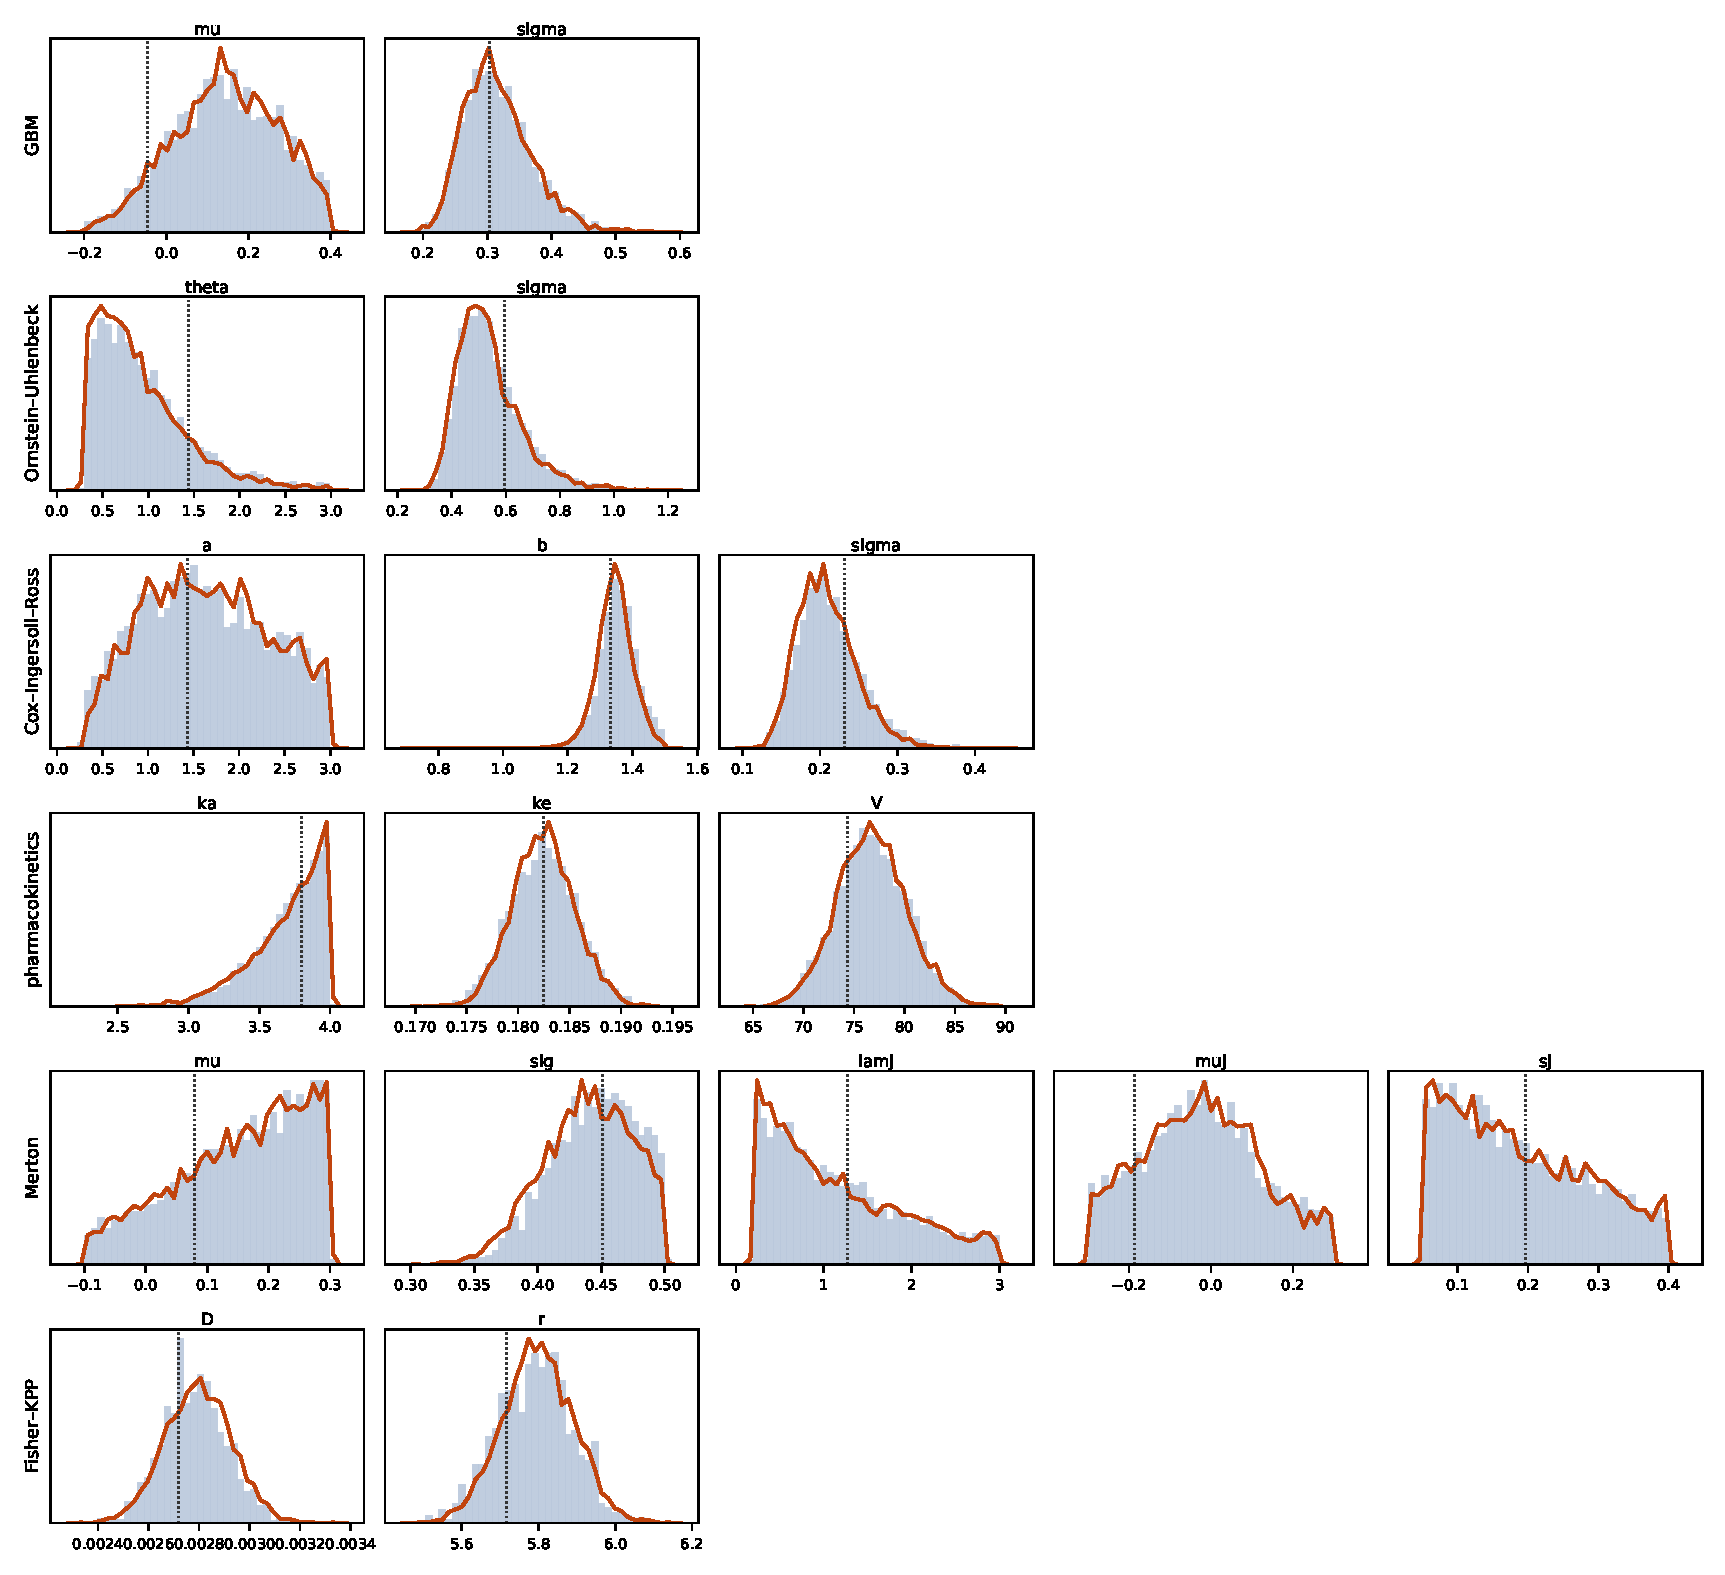
\includegraphics[width=\linewidth,height=0.82\textheight,keepaspectratio]{figs/marginals_muon.pdf}
\caption{\textbf{Posterior marginals}, model (line) against reference (filled), for every system of
Table~\ref{tab:main}. Each panel shows the median-$\FIDsd$ test instance of its system, with $4{,}000$
draws per side. The dotted line is at the generating parameter. The axis of each panel spans its
sample range, not the prior box (Fig.~\ref{fig:pairs} shows the prior-relative scale). Rows are
systems, columns their parameters. This is the same comparison that the table reduces to one number
per cell, and it shows what that number cannot: the model is exact on linear-Gaussian, GBM and double
well, and faithful but slightly over-dispersed on the other systems. On Lotka--Volterra's $\beta$ and
on Hodgkin--Huxley's conductances on sharp instances, a single coordinate carries the whole error.}
\label{fig:marginals}
\end{figure}

\begin{figure}[!htbp]
\centering
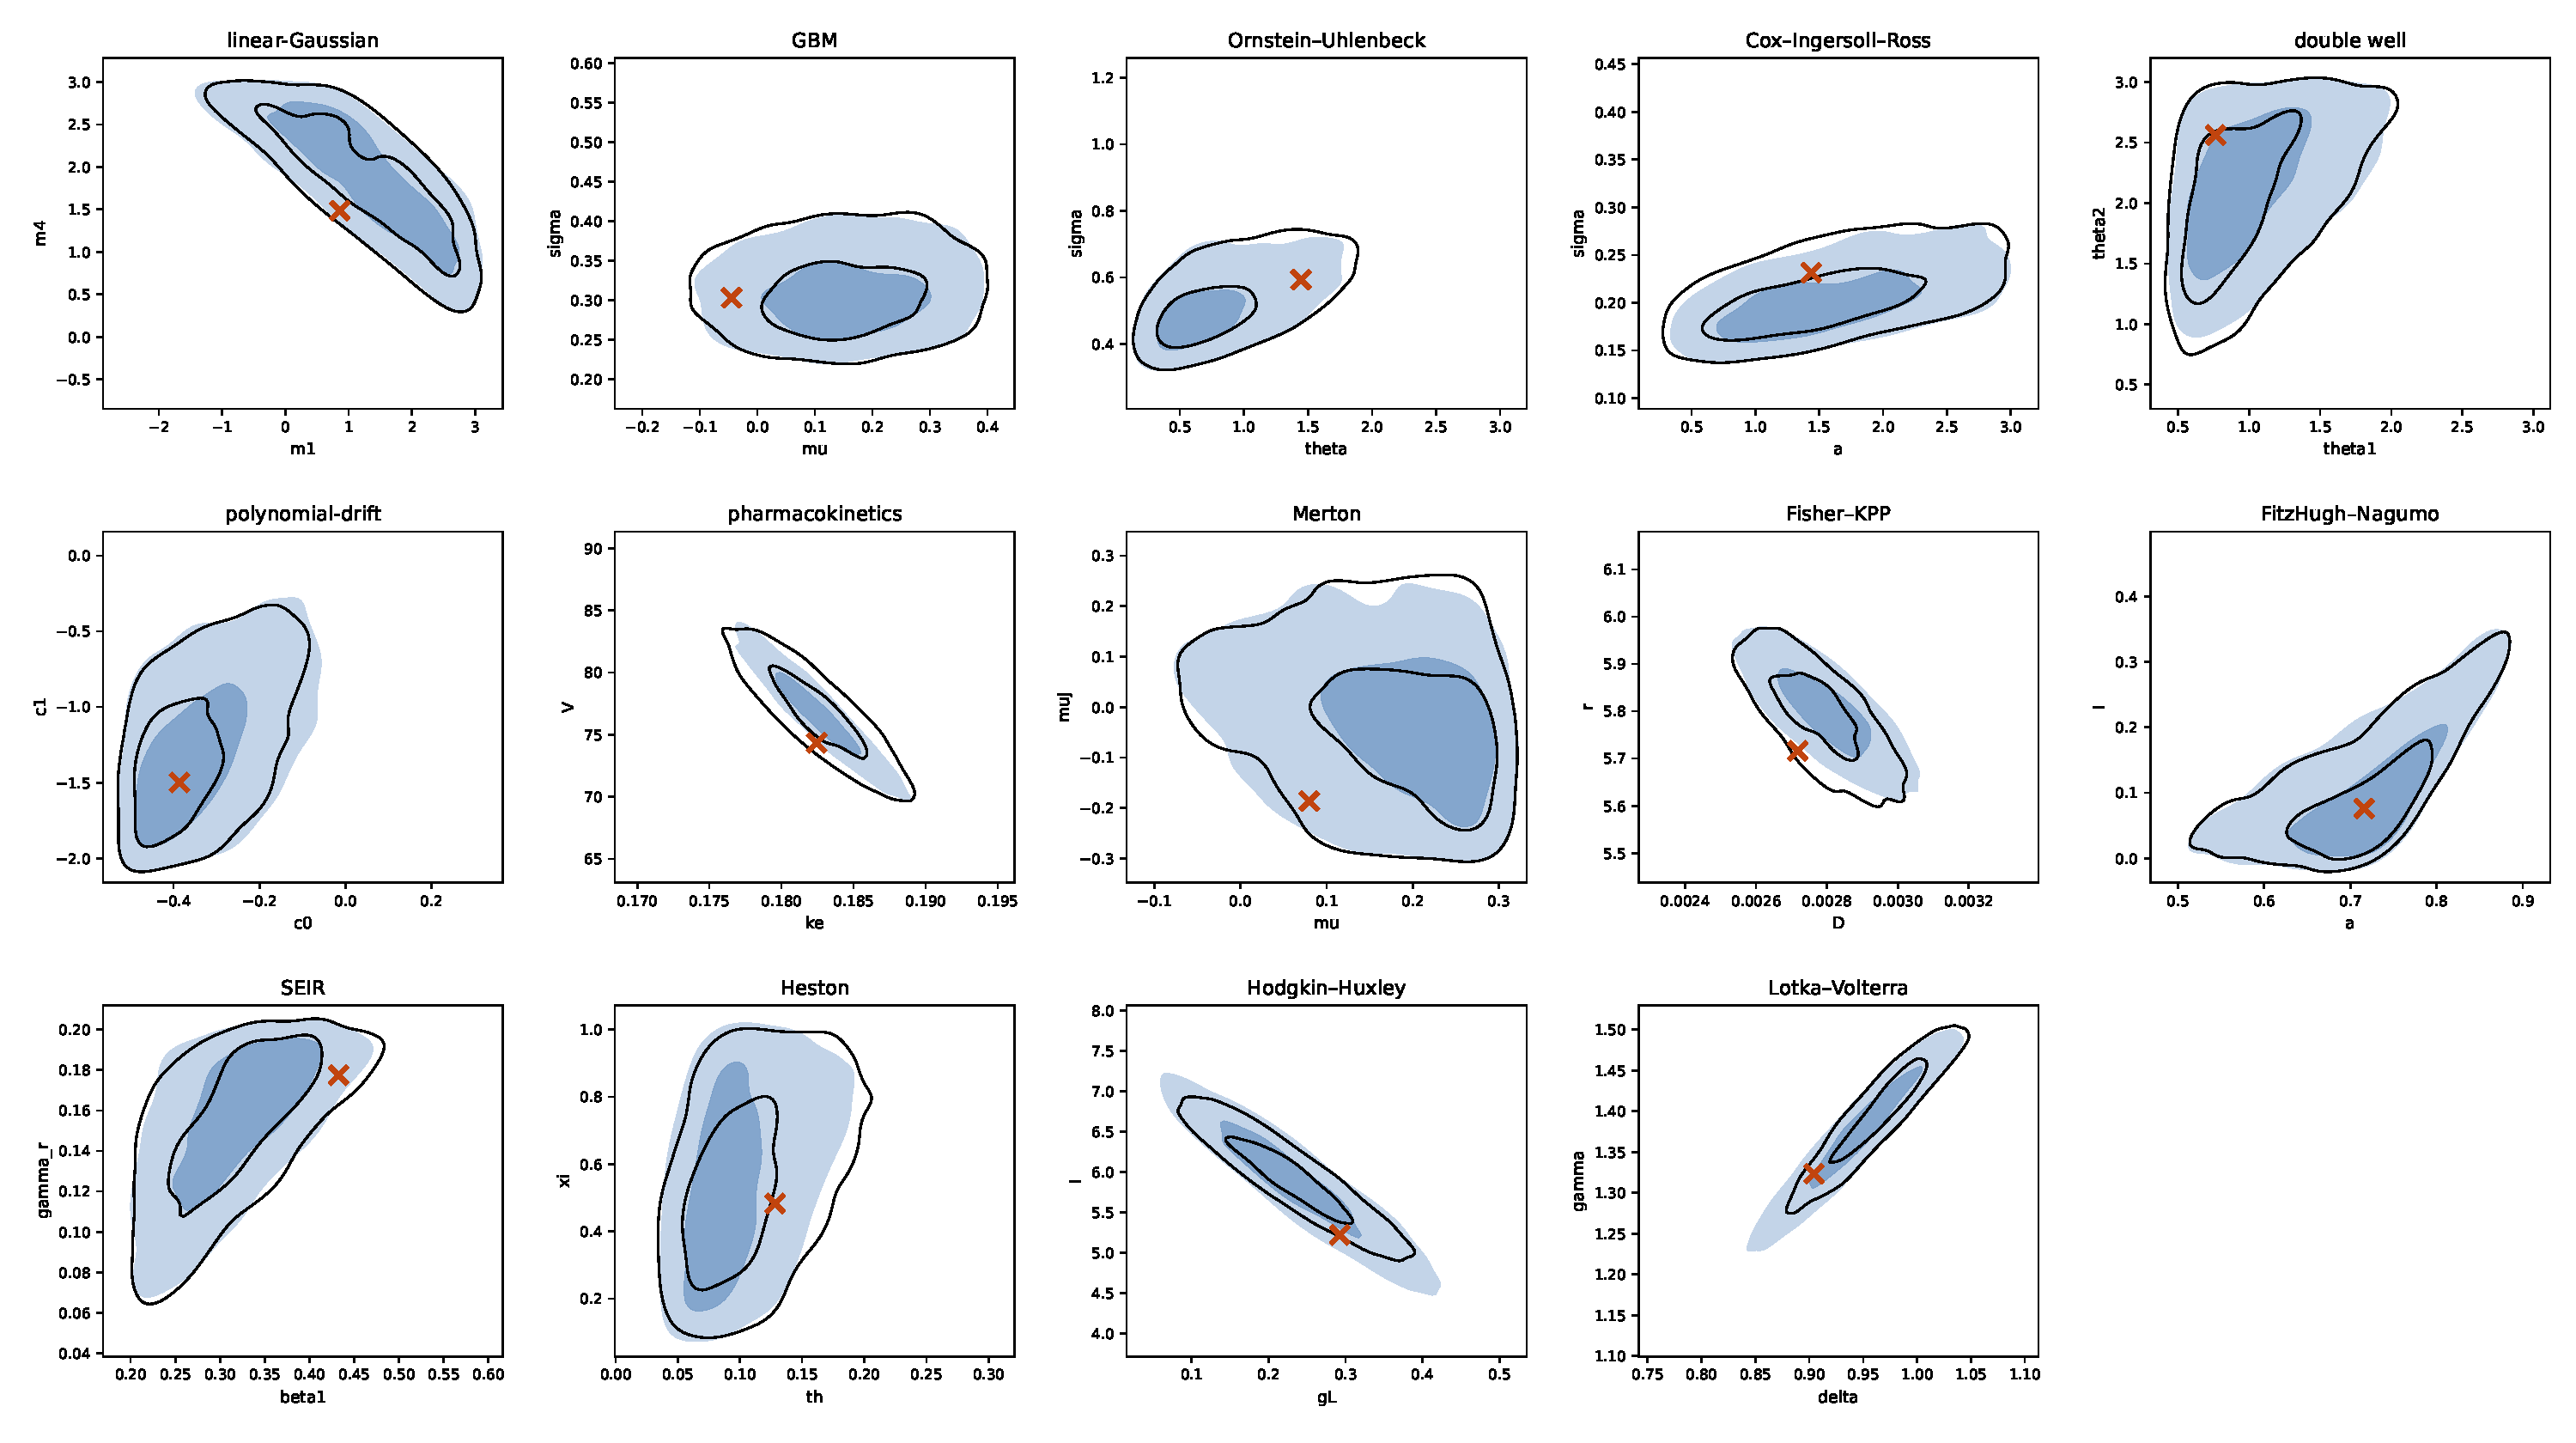
\includegraphics[width=\linewidth,height=0.82\textheight,keepaspectratio]{figs/pairs_muon.pdf}
\caption{\textbf{Joint posteriors} of \amortix\ (filled contours: 39\% and 86\% highest-density
regions) against exact or validated reference posteriors (open contours, same levels). Each panel is
the median-$\FIDsd$ test instance of one system of Table~\ref{tab:main}, from the big model of the
package recipe, with $4{,}000$ draws per side. The cross marks the true parameters. Each panel shows
the most correlated parameter pair of that system, so the comparison is of the shape of the dependence
and not only of the marginal spread. Axes span the sample range of each panel, not the prior box. The
prior is $4$--$107\times$ wider than the posterior standard deviation across the panels shown, and the
sharp FitzHugh--Nagumo and Hodgkin--Huxley instances of Sec.~\ref{sec:refs} reach ${\sim}230\times$.
The plotted shapes carry no information about absolute sharpness.}
\label{fig:pairs}
\end{figure}

We make the following observations. On GBM every size from tiny up sits within two floors of the
resolution of the evaluation set ($0.0028$--$0.0036$ against $0.0018$). Linear-Gaussian, double well
and SEIR land within a few floors at the larger sizes. Those cells bound the error from above and do
not measure it. Ornstein--Uhlenbeck (${\sim}0.028$) and Cox--Ingersoll--Ross ($0.07$--$0.08$) do not
depend on the model size; their residuals belong to the task, not to capacity or recipe.
FitzHugh--Nagumo and Hodgkin--Huxley improve most strongly with model size ($0.45 \to 0.036$ from pico
to small, $9.8 \to 0.31$ across the five sizes, with the largest model still improving), and they
carry the largest residuals of the suite. The stochastic Lotka--Volterra residual ($0.80$) sits almost
entirely in one coordinate (Fig.~\ref{fig:marginals}), and capacity does not explain it ($0.95$ at
the big size). Validated stopping has a measurable effect: under the margin rule of
Sec.~\ref{sec:recipe}, the best-on-validation checkpoint replaced the final weights in half of the
$194$ training runs behind Table~\ref{tab:main}, in 13 of 15 runs on Cox--Ingersoll--Ross and in 15
of 15 on FitzHugh--Nagumo (Appendix~\ref{app:optmeas}).

Figure~\ref{fig:pairs} shows the object the package produces, the joint posterior itself, on the
median-error test instance of every reference-block system, model against reference. The recipe and
the checkpoints are those of Table~\ref{tab:main}.

\subsection{Amortization over observation designs}
\label{sec:design-amortization}

The central claim of the package is that one trained network answers $p(m \mid S)$ for \emph{every}
observation design $S$, at any number and placement of points. Fig.~\ref{fig:fidk} tests this claim
on the six systems of the suite where a per-design reference can be computed and validated. Each test
observation set draws a fresh random design, the reference posterior is recomputed on exactly those
points, and FID is evaluated per design-size bucket. In our experiments, amortization over designs is
not a trade-off against accuracy. The stars in Fig.~\ref{fig:fidk} are networks trained on a single
fixed design; wherever such a network exists, the amortized network is comparable to it at that design
size, and only the amortized network answers anywhere else on the $K$ axis. It also removes a failure
mode, because the resampling of the observation subset at every optimizer step is also a data
augmentation. The two systems with elevated FID are not noise, and we analyze them next.

\begin{figure}[!htbp]
\centering
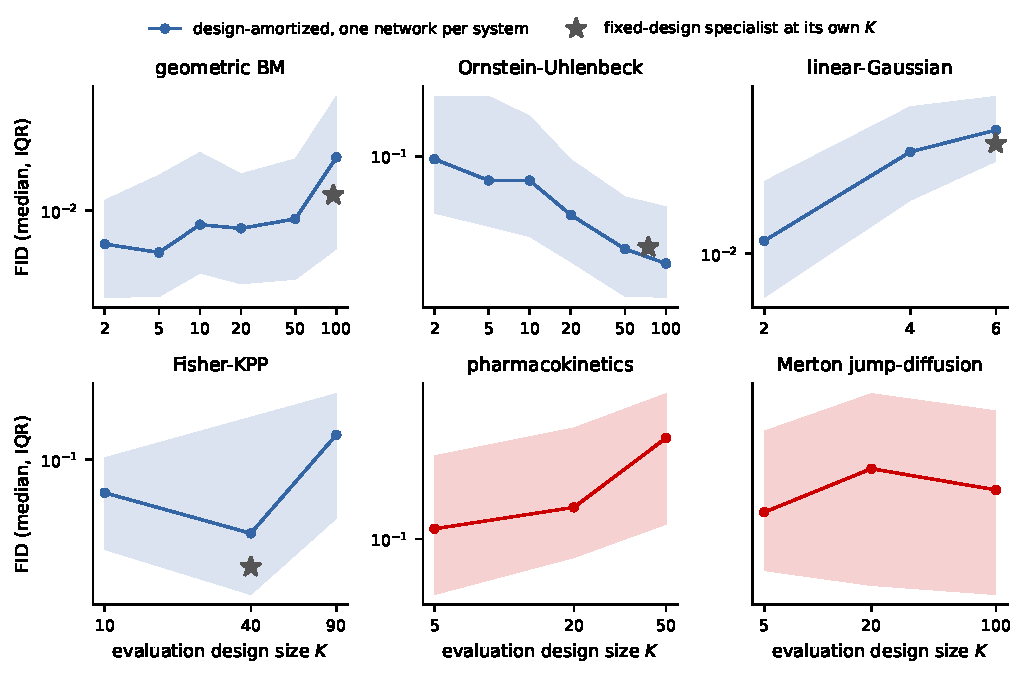
\includegraphics[width=0.98\linewidth]{figs/fid_vs_k.pdf}
\caption{\textbf{FID vs.\ design size}, for one design-amortized network per system. The line is the
median and the band is the interquartile range over the test observation sets of each bucket. A
bucket has $100$ sets for GBM, OU and linear-Gaussian, and $32$ for the MCMC-referenced systems. Each
set has a fresh random design and a per-design reference recomputed on exactly those points. These are
the six systems whose references were built on a grid of design sizes; the rest of the suite has
references at one design size (Table~\ref{tab:main}), which scores a model but does not trace a curve.
Stars: networks of the same architecture trained on a single fixed design. They exist only at their
own $K$ and are shown for context. The Merton and pharmacokinetics curves use the converged references
of Sec.~\ref{sec:refs}. The text analyzes the pharmacokinetic rise with $K$, which is the precision
floor. Both axes are logarithmic. Note the different vertical scales.}
\label{fig:fidk}
\end{figure}

\paragraph{Why $\FIDsd$ rises with the design size.} $\FIDsd$ is a ratio. On pharmacokinetics
($0.07 \to 0.34$ from $K = 5$ to $50$, Fig.~\ref{fig:fidk}) only its denominator moves. We measured
this on the same evaluation sets, in prior-range units. The absolute posterior-mean error of the
network is flat in $K$ ($\varepsilon_\Delta = 1$--$12 \times 10^{-3}$, no trend), while the reference
posterior contracts by the $\sqrt{K}$ of a regular model (widths fall $2.8$--$5.1\times$, against
$\sqrt{10} \approx 3.2$). The bias term $\sum_i (\varepsilon_{\Delta,i}/w_{\Delta,i})^2$ grows
accordingly, $0.025 \to 0.121$. In the prior normalization the same model reads
$\FIDpr \approx 3 \times 10^{-4}$ at the densest designs, and the posterior widths stay within
$1$--$8\%$ of the reference at every $K$. The network has a fixed localization floor of
$10^{-3}$--$10^{-2}$ of the prior range; what grows is its visibility, once the data determine the
parameters more precisely than that. We therefore report the pharmacokinetic entries per design size
and do not pool them. The narrowest-posterior instances read several times worse than the rest, and a
median over one 32-instance evaluation set moves between $0.04$ and $0.15$ between otherwise
identical training runs. The stochastic systems stay an order of magnitude above the floor even at
$K = 100$. Fisher--KPP approaches the floor only at its densest bucket ($0.126$ at $K = 90$).

\subsection{Cost of training and inference}
\label{sec:cost}

Training under the package recipe ($90{,}000$ steps at batch $512$, $120{,}000$ simulations,
validated stopping) costs $58$--$82$ minutes per system at the small size on one H200 GPU. The big
size costs $67$--$111$ minutes, and Hodgkin--Huxley costs $136$ minutes because its simulator is the
most expensive. The budget is deliberately generous: with the checkpoint chosen by validation,
overshooting it costs time and never quality (Sec.~\ref{sec:recipe}). At a $20{,}000$-simulation
budget training takes $4$--$8$ minutes. The same run on a laptop CPU takes about four times longer
and gives a bit-identical posterior, because all stochastic generation stays on a CPU random number
generator. At inference, $2{,}000$ posterior samples for one observation set cost $72$\,ms batched
($135$\,ms single) on the GPU and $426$\,ms on the laptop CPU, at any design size and placement.

Table~\ref{tab:refcost} sets these numbers against the per-instance cost of the reference engines that
built the evaluation sets, at the settings that built them. The chains are long enough to clear the
two-chain floors of Sec.~\ref{sec:refs}; this is reference grade and not user grade, and a
$2{,}000$-draw exact-likelihood chain costs $42$--$124$\,ms. The comparison cuts both ways. Where the
likelihood costs microseconds, exact-likelihood MCMC gives a user-grade posterior in tens of
milliseconds and a reference-grade one in seconds, which is cheaper than the training of the
amortized network for any realistic number of observation sets. This is why those engines, and not
the network, are the accuracy record of this report. The relation inverts where one likelihood
evaluation is itself a simulation. A Fisher--KPP reference costs $186$\,s (a PDE solve per
evaluation), a SEIR reference $16$ minutes (an epidemic integration per evaluation), a
Hodgkin--Huxley reference a median $18$ minutes of nested sampling, and a double-well or
polynomial-drift reference $38$ minutes of pseudo-marginal MH. At those prices the entire training
run amortizes within a handful of posteriors: two on the double well, four on SEIR and on
Hodgkin--Huxley, and about twenty on Fisher--KPP. Every posterior after that costs $70$\,ms.
Sequential refinement and design search require posteriors by the hundred, and that is the intended
regime of the package.

\begin{table}[t]
\centering
\small
\begin{tabular}{@{}llr@{}}
\toprule
engine & systems & one posterior \\
\midrule
closed form / conjugate & linear-Gaussian, GBM & ${<}1$\,ms \\
Poisson-mixture / log-normal MCMC & Merton, pharmacokinetics & $5$--$7$\,s \\
exact-likelihood MCMC & OU, CIR & $6$--$34$\,s \\
tempered SMC, particle-filter likelihood & Heston & $58$\,s \\
nested sampling (\texttt{dynesty}) & FitzHugh--Nagumo & ${\approx}2$\,min \\
PDE-likelihood MCMC & Fisher--KPP & $186$\,s \\
tempered SMC, bridge likelihood & stochastic Lotka--Volterra & ${\approx}4$\,min \\
exact-likelihood MCMC & SEIR & ${\approx}16$\,min \\
nested sampling (\texttt{dynesty}) & Hodgkin--Huxley & ${\approx}18$\,min \\
pseudo-marginal MH, bridge likelihood & double well, polynomial-drift & ${\approx}38$\,min \\
\midrule
\amortix\ small (GPU), after training & any of the above & $0.07$\,s \\
\amortix\ small (laptop CPU) & & $0.43$\,s \\
\bottomrule
\end{tabular}
\caption{\textbf{Cost of one reference posterior} per instance, at the settings that built the frozen
evaluation sets. MCMC rows are single chains of $1.5$--$2 \times 10^5$ draws (Fisher--KPP $4{,}000$;
double well and polynomial drift $60{,}000$ pseudo-marginal draws), thinned to the $4{,}000$ stored
draws. The two-chain admission of Sec.~\ref{sec:refs} runs each engine two to three times. Every
engine runs on the CPU, with one to a few threads on one server core, except the Heston SMC filter,
which runs on the GPU at the production population of $16{,}384$ $\theta$-particles over a $4{,}096$-particle
filter (median over $96$ runs, spread $28$--$144$\,s). The CPU chains are single-instance timings. The
dynesty rows are medians over the $32$ test instances, reconstructed from the per-job wall times of
the reference builds (\texttt{nlive}${=}1000$); the spread across instances is about four on
FitzHugh--Nagumo and about twenty on Hodgkin--Huxley, and the hardest Hodgkin--Huxley instances take
one hour. Training the amortized network costs $58$--$82$ minutes on one H200 GPU (text above). After
training, one posterior costs the entry in the last two rows.}
\label{tab:refcost}
\end{table}

\section{Discussion and limitations}
\label{sec:discussion}

Our results support one specific claim. For dynamical-systems inverse problems, the input
representation of an amortized posterior estimator is the dominant accuracy factor, not a
preprocessing detail, and it can be part of the model rather than part of the problem specification.
With prescribed coordinates our own estimator acquires the failures of Sec.~\ref{sec:features}. The
learnable representation removes them with one configuration for all fourteen systems, and the
reference posteriors of Sec.~\ref{sec:protocol} certify the result.

\paragraph{Limitations.} Bayesian experimental design, the intended consumer of design amortization,
is not demonstrated yet; the training procedure of Sec.~\ref{sec:recipe} makes the required object
$p(m \mid S)$ coherent across subsets $S$. No real-data study with posterior predictive checks is
included. Priors are limited to factorized distributions with tractable marginal CDFs, the class the
probit map \eqref{eq:probit} covers; correlated priors need a different normalization, and priors with
atoms at zero, which would admit a sparse-coefficient variant of the polynomial-drift system, are a
planned extension. The two hardest systems are not at reference quality. Hodgkin--Huxley still
improves at the largest model size, and capacity does not explain the Lotka--Volterra residual
(Sec.~\ref{sec:summary}), which is the clearest open problem in the suite. One more limitation
concerns the sampler. The uniform time grid of these measurements does not resolve posteriors much
narrower than the prior (Sec.~\ref{sec:recipe}). The numbers of this report are not affected, because
the posteriors of the suite are wide enough; numbers on sharper problems measured with that grid are
lower bounds on the quality of the model.

\appendix

\section{Controls and calibration screen}
\label{app:systems}

\paragraph{Controls.}
\label{sec:baselines-tiers}
Two model-free controls accompany every result. The \emph{prior-mean predictor} ignores the data
(exactly $25\%$ mean absolute error under a uniform prior). The \emph{ridge control} is a point
predictor of the parameters: a degree-2 ridge regression on generic summary statistics of the token
set, namely, per token feature, the mean, the standard deviation, the mean square, the mean absolute
value and the $0.1/0.5/0.9$ quantiles, computed over the observations that are present. It recovers
no distribution and is not meant to. Its role is to detect one silent failure that the calibration
screen cannot see: a posterior that ignores the data and returns the prior passes SBC perfectly, and
only a point-accuracy control unmasks it.

\paragraph{Calibration of the fixed-grid gallery.}

Table~\ref{tab:pvals} lists the per-parameter SBC $p$-values of the standard-budget gallery run
($40{,}000$ simulations). The protocol is as follows. For each system, 500 synthetic observation sets
are simulated with known parameters. For each observation set the model gives 200 posterior draws,
and the rank of the true parameter among the draws is recorded. A calibrated posterior gives uniform
ranks, and each $p$-value tests this uniformity for one parameter. All parameters pass except
Cox--Ingersoll--Ross $b$, whose deviation corresponds to a location shift of the posterior in $b$ of
$\approx 0.15$~sd, the largest calibration deviation in the gallery.

\begin{table}[t]
\centering
\footnotesize
\begin{tabular}{@{}ll@{}}
\toprule
system & per-parameter SBC $p$-values \\
\midrule
linear-Gaussian & $m_1$: 0.06 \quad $m_2$: 0.60 \quad $m_3$: 0.38 \quad $m_4$: 0.56 \\
Ornstein--Uhlenbeck & $\theta$: 0.28 \quad $\sigma$: 0.77 \\
SEIR & $\beta_1$: 0.33 \quad $\beta_2$: 0.22 \quad $\alpha$: 0.61 \quad $\gamma_r$: 0.34 \quad $\gamma_d$: 0.53 \\
geometric Brownian motion & $\mu$: 0.26 \quad $\sigma$: 0.44 \\
Cox--Ingersoll--Ross & $a$: 0.65 \quad $b$: \textbf{0.001} \quad $\sigma$: 0.73 \\
double well & $\theta_1$: 0.78 \quad $\theta_2$: 0.54 \quad $\sigma$: 0.88 \\
stochastic Lotka--Volterra & $\alpha$: 0.07 \quad $\beta$: 0.69 \quad $\delta$: 0.08 \quad $\gamma$: 0.35 \\
FitzHugh--Nagumo & $a$: 0.19 \quad $b$: 0.15 \quad $\epsilon$: 0.90 \quad $I$: 0.63 \\
polynomial-drift SDE & $c_0$: 0.06 \quad $c_1$: 0.96 \quad $c_2$: 0.46 \quad $c_3$: 0.80 \quad $\sigma$: 0.50 \\
\bottomrule
\end{tabular}
\caption{\textbf{Calibration screen.} Per-parameter SBC uniformity $p$-values for the standard-budget
fixed-design gallery run (500 observation sets $\times$ 200 draws; $p > 0.05$ passes). The single
failure is in bold.}
\label{tab:pvals}
\end{table}

\section{Optimizer and stopping-rule measurements}
\label{app:optmeas}

\paragraph{Setup.} Every number in this appendix comes from one configuration, so that only the
optimizer variables change. The system is the design-amortized GBM, the model is the big one ($2.3$M
parameters), and the score is $\FIDsd$ against the exact conjugate reference on a fixed six-bucket
evaluation set. The design sizes are $K = 2, 5, 10, 20, 50, 95$, with $32$ observation sets per bucket
and two-chain floors of $0.0012$--$0.0019$. Reported values are means over the six buckets. Each
training run occupies one H200 GPU. Several comparisons hold the example budget (batch $\times$ steps)
fixed on purpose and say so.

\paragraph{Step size at the reference batch.} At batch $512$ and $9{,}000$ steps ($4.6$M examples):

\begin{center}
\small
\begin{tabular}{@{}lcccccc@{}}
\toprule
Muon step $\eta$ & $3\times10^{-4}$ & $10^{-3}$ & $3\times10^{-3}$ & $10^{-2}$ & $2\times10^{-2}$ & $6\times10^{-2}$ \\
\midrule
$\FIDsd$ & $0.0133$ & $0.0070$ & $0.0065$ & $0.0061$ & $0.0085$ & diverges \\
\bottomrule
\end{tabular}
\end{center}

The basin is broad and shallow between $3\times10^{-3}$ and $10^{-2}$, and the edge beyond it is
hard. The package value is $10^{-2}$.

\paragraph{Scaling with batch size.} We repeated the sweep at batches $64$, $2{,}048$ and $8{,}192$,
with the example budget fixed within each comparison. The optimum is at $3.5\times10^{-3}$, $10^{-2}$
(flat to $2\times10^{-2}$) and $2\times10^{-2}$. From batch 64 to 512 the optimum moves by
$\times2.82$, against $\times2.83$ predicted by $\sqrt{B}$. The fourth-root alternative is excluded,
not only disfavored: its prediction costs $0.0079$ against $0.0066$ at batch 64. Past batch
${\sim}2{,}048$ the optimum stops moving. At $8{,}192$ the square root would extrapolate to
$4\times10^{-2}$, which scores worse than the capped $2\times10^{-2}$ ($0.0060$ against $0.0052$),
and twice the extrapolation diverges. Hence the rule of Sec.~\ref{sec:recipe}:
$\eta(B) = \min\bigl(10^{-2}\sqrt{B/512},\ 2\times10^{-2}\bigr)$, square root below the critical
batch, constant above it.

\paragraph{Transfer across width.} At batch 512 and fixed budget, we compare the step $10^{-2}$ with
the hotter $2\times10^{-2}$ across three widths: tiny $0.0089$ vs.\ $0.0087$, small $0.0066$ vs.\
$0.0076$, big $0.0061$ vs.\ $0.0085$. At the hotter step the accuracy is non-monotone in model size
(big is worse than small); at the step of the rule it follows the capacity. ``Wider is worse'' can
therefore be a statement about one number inside the optimizer and not about capacity.

\paragraph{Steps against examples.} At a fixed budget of $9.2$M examples, batch $512 \times 18{,}000$
steps reads $0.0051$, batch $2{,}048 \times 4{,}500$ reads $0.0045$, and batch
$8{,}192 \times 1{,}125$ collapses to $0.0076$. At the same batch and step size, twice the steps
($2{,}020$) recovers $0.0060$. Above a step floor the example budget governs the quality; below it no
example budget helps. The floor is per-system and spans an order of magnitude: the pharmacokinetic
validation curve reaches its optimum near $66{,}000$ steps at batch 512, while the GBM curve shows no
interior optimum up to $36{,}000$. This motivates validated stopping in place of per-system budgets.

\paragraph{Validated stopping.} The resolution of the monitor must be evaluated at the sample count
of the monitor itself. The GBM validation set resolves $0.0013$ at $4{,}000$ draws but only $0.0044$
at $1{,}000$. We measured both failure modes of the naive keep-the-best rule before we adopted the
margin. A monitor coarser than its model ships the deepest noise dip: $0.0053$ on test against
$0.0040$ for the final weights. A resolving monitor still ships $0.0052$, because under a cosine
schedule the mid-run checkpoints are systematically inflated, and an argmin over the whole curve
mistakes that for a reversal. The margin rule accepts the best checkpoint only when it improves on
the final weights by more than the resolution of the monitor, and it passes both cases. A genuine late
reversal clears it by an order of magnitude: on pharmacokinetics the validation curve turns from
$0.1066$ at step $66{,}222$ to $0.1321$ at $72{,}072$, which is twenty floors, and the selected
checkpoint recovers the difference.

\section{Reference posteriors}
\label{app:refs}

\paragraph{GBM conjugate posterior.} With observations at indices $i_0 = 0 < i_1 < \dots$ of the fine
grid, the log-returns $r_k = \log(S_{i_{k+1}}/S_{i_k})$ over gaps $\tau_k$ are independent
$\N\bigl((\mu - \sigma^2/2)\tau_k, \sigma^2 \tau_k\bigr)$. In the coordinates
$(b, \sigma^2) = (\mu - \sigma^2/2, \sigma^2)$ the model is a Gaussian location--scale family with
sufficient statistics $T = \sum_k \tau_k$, $R_1 = \sum_k r_k$ and
$SS_w = \sum_k r_k^2 / \tau_k - R_1^2 / T$. Draws from the standard conjugate posterior
($\sigma^2 = SS_w / \chi^2_{n-1}$, $b \mid \sigma^2 \sim \N(R_1/T, \sigma^2/T)$) are transformed to
$(\mu, \sigma)$ and importance-resampled to the uniform box prior with the Jacobian weight. We
validated the sampler against exact-likelihood MCMC on the same designs: over 24 comparisons, the
worst posterior-mean discrepancy is $0.099$~sd and the width ratios are $0.91$--$1.03$.

\paragraph{Adaptive Metropolis.} Random-walk Metropolis on the box, with proposal
$x' = x + s\,C\,\xi$, $\xi \sim \N(0, I)$. During burn-in ($\max(500, n/2)$ iterations) the scalar $s$
adapts toward a $0.25$ acceptance rate in blocks of 50 with a decaying Robbins--Monro gain. Once
enough burn-in states are collected, the Cholesky factor of the empirical covariance, rescaled by
$2.38/\sqrt{d}$, replaces the shape $C$ \citep{haario2001}. Adaptation is frozen for the retained
phase. Out-of-box proposals are rejected, which samples the box-truncated target exactly because the
proposal is symmetric. The likelihoods are as follows. OU uses per-gap Euler--Maruyama Gaussian
transitions, which match the generative process, plus the stationary density of $X_0$. GBM uses the
exact log-return density. Merton uses the Poisson-mixture transition density, truncated at the
numerically negligible jump count. Pharmacokinetics uses log-normal residuals around the Bateman
curve. Fisher--KPP uses a Gaussian observation model around the deterministic PDE solve. Every chain
used as a reference is paired with a second chain from a well-separated start, and the between-chain
posterior-mean discrepancies are reported next to the results they certify.

\paragraph{Nested sampling, SMC, and particle-filter likelihoods.} FitzHugh--Nagumo and
Hodgkin--Huxley references come from \texttt{dynesty} (static nested sampling; the prior transform is
the uniform box; \texttt{nlive}${=}1000$). The admission partner runs \texttt{nlive}${=}2000$ from an
independent seed, and the pair must agree below the two-chain threshold of Sec.~\ref{sec:refs}.
Stochastic Lotka--Volterra and Heston use adaptive tempered SMC \citep{delmoral2006}: the
inverse-temperature step is chosen at each stage so that the effective sample size stays at half the
population, followed by systematic resampling and random-walk rejuvenation at the current temperature.
Admission is by population doubling ($N$ against $2N$ from independent seeds). Their likelihoods are
unbiased Monte-Carlo estimates: Lotka--Volterra uses a Durham--Gallant bridge sampler
\citep{durham2002}, and Heston uses a bootstrap particle filter that runs the clamped-Euler update of
the simulator itself (Sec.~\ref{sec:refs}). The particle counts keep the spread of the estimator at
fixed parameters to a fraction of a nat. Double well and polynomial drift use the same bridge
estimator inside the pseudo-marginal variant \citep{andrieu2010} of the adaptive Metropolis sampler
above.

\section{Correspondence with package options}
\label{app:package}

\begin{center}
\small
\begin{tabular}{@{}ll@{}}
\toprule
in this report & in the package \\
\midrule
point tokens & \texttt{embed="wpoint"} \\
pair tokens + set conditioning & \texttt{embed="wfilm"} \\
warped values/increments (fixed designs) & \texttt{embed="wbasis"} / \texttt{"wdiff"} \\
attention phases from physical time & \texttt{rope="time"} \\
value coordinate of the token (raw or log) & \texttt{DesignProblem.value\_coord}, required \\
fresh designs each optimizer step & \texttt{fit(retokenize=...)} via \texttt{make\_retokenizer()} \\
Muon with the batch step law & \texttt{fit(optimizer="muon")}; \texttt{muon\_lr=None} $\to$ the measured law \\
validated stopping with margin & \texttt{fit(keep\_best=True, monitor\_floor=...)} \\
sampler steps, scheme and time grid & \texttt{sample(n=, n\_steps=, solver=, t\_grid=)}, all required \\
evaluation-set resolution at $n$ draws & \texttt{evaluation.floor\_at} \\
variable-design problem wrapper & \texttt{amortix.designs.DesignProblem} \\
benchmark systems & \texttt{amortix.problems} (\texttt{DESIGN\_ZOO}) \\
calibration screen & \texttt{sbc\_design} \\
reference machinery & \texttt{amortix.mcmc}, \texttt{.smc}, \texttt{.bridgelik}, \texttt{.hestonlik} + likelihood factories \\
\bottomrule
\end{tabular}
\end{center}

\texttt{FlowPosterior(problem)} selects the embedding and the attention phases from the problem class.
The settings that decide the result of a sampling call have no default values: the number of draws,
the number of ODE steps, the scheme and the time grid are named in every call, and the coordinate of
the observed value is declared by the problem class. The non-default architecture options remain in
the package as reproducible controls.

\clearpage
\setlength{\bibsep}{0.9pt plus 0.2ex}
\begin{thebibliography}{28}
\small\setlength{\itemsep}{0.9pt}\setlength{\parskip}{0pt}

\bibitem[Andrieu et al.(2010)]{andrieu2010} C.~Andrieu, A.~Doucet, R.~Holenstein.
Particle Markov chain Monte Carlo methods. \emph{JRSS B} 72(3), 2010.

\bibitem[Boelts et al.(2024)]{boelts2024} J.~Boelts, M.~Deistler, M.~Gloeckler, et al.
sbi reloaded: a toolkit for simulation-based inference workflows. \emph{arXiv:2411.17337}, 2024.

\bibitem[Brunton et al.(2016)]{brunton2016} S.~L.~Brunton, J.~L.~Proctor, J.~N.~Kutz.
Discovering governing equations from data by sparse identification of nonlinear dynamical systems.
\emph{PNAS} 113(15), 2016.

\bibitem[Clerx et al.(2019)]{clerx2019} M.~Clerx, M.~Robinson, B.~Lambert, C.~L.~Lei,
S.~Ghosh, G.~R.~Mirams, D.~J.~Gavaghan. Probabilistic inference on noisy time series (PINTS).
\emph{Journal of Open Research Software} 7(1), 2019.

\bibitem[Cox et al.(1985)]{cox1985} J.~C.~Cox, J.~E.~Ingersoll, S.~A.~Ross.
A theory of the term structure of interest rates. \emph{Econometrica} 53(2), 1985.

\bibitem[Cranmer et al.(2020)]{cranmer2020} K.~Cranmer, J.~Brehmer, G.~Louppe.
The frontier of simulation-based inference. \emph{PNAS} 117(48), 2020.

\bibitem[Darcet et al.(2024)]{darcet2024} T.~Darcet, M.~Oquab, J.~Mairal, P.~Bojanowski.
Vision transformers need registers. \emph{ICLR}, 2024.

\bibitem[Del Moral et al.(2006)]{delmoral2006} P.~Del Moral, A.~Doucet, A.~Jasra.
Sequential Monte Carlo samplers. \emph{JRSS B} 68(3), 2006.

\bibitem[Durham and Gallant(2002)]{durham2002} G.~B.~Durham, A.~R.~Gallant. Numerical
techniques for maximum likelihood estimation of continuous-time diffusion processes.
\emph{Journal of Business \& Economic Statistics}, 20(3):297--338, 2002.

\bibitem[FitzHugh(1961)]{fitzhugh1961} R.~FitzHugh. Impulses and physiological states in
theoretical models of nerve membrane. \emph{Biophysical Journal} 1(6), 1961.

\bibitem[Gabrielsson and Weiner(2000)]{gabrielsson2000} J.~Gabrielsson, D.~Weiner.
\emph{Pharmacokinetic and Pharmacodynamic Data Analysis: Concepts and Applications}. Swedish
Pharmaceutical Press, 2000.

\bibitem[Gloeckler et al.(2024)]{gloeckler2024} M.~Gloeckler, M.~Deistler, C.~Weilbach, F.~Wood,
J.~H.~Macke. All-in-one simulation-based inference. \emph{ICML}, 2024.

\bibitem[Greenberg et al.(2019)]{greenberg2019} D.~Greenberg, M.~Nonnenmacher, J.~Macke.
Automatic posterior transformation for likelihood-free inference. \emph{ICML}, 2019.

\bibitem[Haario et al.(2001)]{haario2001} H.~Haario, E.~Saksman, J.~Tamminen.
An adaptive Metropolis algorithm. \emph{Bernoulli} 7(2), 2001.

\bibitem[Hermans et al.(2022)]{hermans2022} J.~Hermans, A.~Delaunoy, F.~Rozet, A.~Wehenkel,
V.~Begy, G.~Louppe. A trust crisis in simulation-based inference? Your posterior approximations can be
unfaithful. \emph{TMLR}, 2022.

\bibitem[Heston(1993)]{heston1993} S.~L.~Heston. A closed-form solution for options with stochastic
volatility with applications to bond and currency options. \emph{Rev.\ Financial Studies} 6(2), 1993.

\bibitem[Hodgkin and Huxley(1952)]{hodgkin1952} A.~L.~Hodgkin, A.~F.~Huxley.
A quantitative description of membrane current and its application to conduction and excitation in
nerve. \emph{J.\ Physiology} 117(4), 1952.

\bibitem[Horn et al.(2020)]{horn2020} M.~Horn, M.~Moor, C.~Bock, B.~Rieck, K.~Borgwardt.
Set functions for time series. \emph{ICML}, 2020.

\bibitem[Jordan et al.(2024)]{jordan2024} K.~Jordan, Y.~Jin, V.~Boza, J.~You, F.~Cesista,
L.~Newhouse, J.~Bernstein. Muon: an optimizer for hidden layers in neural networks, 2024.
\texttt{kellerjordan.github.io/posts/muon}.

\bibitem[Lipman et al.(2023)]{lipman2023} Y.~Lipman, R.~T.~Q.~Chen, H.~Ben-Hamu, M.~Nickel, M.~Le.
Flow matching for generative modeling. \emph{ICLR}, 2023.

\bibitem[Lueckmann et al.(2021)]{lueckmann2021} J.-M.~Lueckmann, J.~Boelts, D.~Greenberg,
P.~Gon\c{c}alves, J.~Macke. Benchmarking simulation-based inference. \emph{AISTATS}, 2021.

\bibitem[Merton(1976)]{merton1976} R.~C.~Merton. Option pricing when underlying stock returns are
discontinuous. \emph{J.\ Financial Economics} 3(1--2), 1976.

\bibitem[Nagumo et al.(1962)]{nagumo1962} J.~Nagumo, S.~Arimoto, S.~Yoshizawa. An active
pulse transmission line simulating nerve axon. \emph{Proceedings of the IRE} 50(10), 1962.

\bibitem[Papamakarios and Murray(2016)]{papamakarios2016} G.~Papamakarios, I.~Murray.
Fast $\epsilon$-free inference of simulation models with Bayesian conditional density estimation.
\emph{NeurIPS}, 2016.


\bibitem[Peebles and Xie(2023)]{peebles2023} W.~Peebles, S.~Xie.
Scalable diffusion models with transformers. \emph{ICCV}, 2023.

\bibitem[Perez et al.(2018)]{perez2018} E.~Perez, F.~Strub, H.~de~Vries, V.~Dumoulin, A.~Courville.
FiLM: Visual reasoning with a general conditioning layer. \emph{AAAI}, 2018.

\bibitem[Radev et al.(2020)]{radev2020} S.~T.~Radev, U.~K.~Mertens, A.~Voss, L.~Ardizzone, U.~K\"othe.
BayesFlow: Learning complex stochastic models with invertible neural networks.
\emph{IEEE Trans.\ Neural Netw.\ Learn.\ Syst.} 33(4), 2020.

\bibitem[Shukla and Marlin(2021)]{shukla2021} S.~N.~Shukla, B.~M.~Marlin.
Multi-time attention networks for irregularly sampled time series. \emph{ICLR}, 2021.

\bibitem[Skilling(2006)]{skilling2006} J.~Skilling. Nested sampling for general Bayesian
computation. \emph{Bayesian Analysis} 1(4), 2006.

\bibitem[Speagle(2020)]{speagle2020} J.~S.~Speagle. dynesty: a dynamic nested sampling package
for estimating Bayesian posteriors and evidences. \emph{MNRAS} 493(3), 2020.

\bibitem[Su et al.(2024)]{su2024} J.~Su, M.~Ahmed, Y.~Lu, S.~Pan, W.~Bo, Y.~Liu.
RoFormer: Enhanced transformer with rotary position embedding. \emph{Neurocomputing} 568, 2024.

\bibitem[Talts et al.(2018)]{talts2018} S.~Talts, M.~Betancourt, D.~Simpson, A.~Vehtari, A.~Gelman.
Validating Bayesian inference algorithms with simulation-based calibration. \emph{arXiv:1804.06788},
2018.

\bibitem[Wildberger et al.(2023)]{wildberger2023} J.~Wildberger, M.~Dax, S.~Buchholz, S.~R.~Green,
J.~H.~Macke, B.~Sch\"olkopf. Flow matching for scalable simulation-based inference. \emph{NeurIPS},
2023.

\bibitem[Yeo and Johnson(2000)]{yeo2000} I.-K.~Yeo, R.~A.~Johnson.
A new family of power transformations to improve normality or symmetry. \emph{Biometrika} 87(4), 2000.

\end{thebibliography}

\end{document}
